\documentclass[11pt,a4paper]{article}

\usepackage{fontspec}
\defaultfontfeatures{Ligatures=TeX,Scale=MatchLowercase}
\usepackage[italian]{babel}
\usepackage[a4paper,margin=2.4cm]{geometry}
\usepackage{xcolor}
\usepackage{amsmath,amssymb}
\usepackage{microtype}
\usepackage{parskip}
\usepackage{longtable,booktabs,array}
\usepackage{calc}
\usepackage{etoolbox}
\usepackage{graphicx}
\usepackage{caption}
\usepackage{enumitem}
\usepackage{hyperref}
\usepackage{bookmark}
\usepackage{xurl}
\usepackage{fancyhdr}
\usepackage{titlesec}
\usepackage{csquotes}
\usepackage[backend=biber,style=numeric-comp,sorting=nyt,maxbibnames=99,defernumbers=true]{biblatex}
\addbibresource{references/references.bib}

\setcounter{secnumdepth}{1}
\setcounter{tocdepth}{2}
\setlength{\emergencystretch}{3em}
\setlength{\parindent}{0pt}
\setlength{\parskip}{0.55\baselineskip plus 0.15\baselineskip minus 0.1\baselineskip}
\setlength{\LTpre}{0.8\baselineskip}
\setlength{\LTpost}{0.8\baselineskip}
\setlist[itemize]{leftmargin=*,topsep=0.5\baselineskip,itemsep=0.2\baselineskip,parsep=0pt,partopsep=0pt}
\urlstyle{same}
\AtBeginDocument{\renewcommand{\abstractname}{Abstract}}

\titleformat{\section}
  {\normalfont\Large\bfseries}{\thesection}{0.7em}{}
\titlespacing*{\section}{0pt}{0pt}{1.1\baselineskip}
\titleformat{\subsection}
  {\normalfont\large\bfseries}{\thesubsection}{0.65em}{}
\titlespacing*{\subsection}{0pt}{2.2\baselineskip plus 0.4\baselineskip}{0.75\baselineskip}
\titleformat{\subsubsection}
  {\normalfont\normalsize\bfseries}{\thesubsubsection}{0.55em}{}
\titlespacing*{\subsubsection}{0pt}{1.4\baselineskip}{0.35\baselineskip}

\newcounter{none}
\providecommand{\tightlist}{%
  \setlength{\itemsep}{0pt}\setlength{\parskip}{0pt}}

\makeatletter
\patchcmd\longtable{\par}{\if@noskipsec\mbox{}\fi\par}{}{}
\newsavebox\pandoc@box
\newcommand*\pandocbounded[1]{%
  \sbox\pandoc@box{#1}%
  \Gscale@div\@tempa{\textheight}{\dimexpr\ht\pandoc@box+\dp\pandoc@box\relax}%
  \Gscale@div\@tempb{\linewidth}{\wd\pandoc@box}%
  \ifdim\@tempb\p@<\@tempa\p@\let\@tempa\@tempb\fi
  \ifdim\@tempa\p@<\p@\scalebox{\@tempa}{\usebox\pandoc@box}%
  \else\usebox\pandoc@box\fi}
\makeatother

\hypersetup{
  colorlinks=true,
  linkcolor=black,
  urlcolor=blue,
  pdftitle={Documentazione del progetto HPHP},
  pdfauthor={Team Affordance}
}

\pagestyle{fancy}
\fancyhf{}
\fancyhead[L]{Documentazione del progetto HPHP}
\fancyhead[R]{Team Affordance}
\fancyfoot[C]{\thepage}
\setlength{\headheight}{14pt}

\begin{document}

\begin{titlepage}
  \centering
  \vspace*{2cm}
  {\Large Corso di Usability \& User Experience Design\par}
  \vspace{1.5cm}
  {\Huge\bfseries Documentazione del progetto HPHP\par}
  \vspace{0.25cm}
  {\Large\itshape Help People Help People\par}
  \vspace{0.6cm}
  {\LARGE Riprogettazione dell'esperienza di prenotazione sanitaria online\par}
  \vspace{0.45cm}
  {\large CUPweb ed ER Salute\par}
  \vspace{0.9cm}
  \rule{0.58\textwidth}{0.5pt}\par
  \vfill
  {\large Team Affordance\par}
  \vspace{0.4cm}
  Matteo Boscherini\par
  Alessandro Campedelli\par
  Francesco Maria Fuligni\par
  \vfill
  {\large Anno accademico 2025--2026\par}
  \vspace{0.7cm}
  \small Repository del progetto:\\
  \url{https://github.com/MatteMito/UUX-Project}
\end{titlepage}

\begin{abstract}
Il presente elaborato documenta il progetto HPHP (\emph{Help People
Help People}), dedicato alla
riprogettazione dell'esperienza di prenotazione sanitaria online per
CUPweb ed ER Salute della Regione Emilia-Romagna. L'analisi considera le
barriere di accesso digitale degli utenti anziani e il ruolo dei
caregiver familiari, traducendo le evidenze raccolte in requisiti di
progettazione, personas, architettura dell'informazione, wireframe e
protocolli di valutazione. Il lavoro è organizzato in quattro fasi:
ricerca e valutazione, studio di fattibilità, proposta progettuale e
valutazione. Gli artefatti nativi e aggiornabili sono disponibili nel
repository del progetto:\\
\url{https://github.com/MatteMito/UUX-Project}

\textbf{Parole chiave:} sanità digitale; accessibilità; utenti anziani;
caregiver; user experience; prenotazione sanitaria.
\end{abstract}

\subsection*{Materiali supplementari}
Il report è corredato dagli artefatti progettuali mantenuti nei rispettivi
formati nativi e modificabili: il \emph{service blueprint}, i wireframe
delle versioni 0 e 1, il confronto prima/dopo, la checklist delle linee
guida e le schede di personas e cast. I materiali sono organizzati nelle
cartelle delle singole fasi e sono disponibili nel repository del progetto.

\clearpage
\tableofcontents

% !TEX root = ../hphp-project-report.tex
% Generated from HPHP_Documentazione_Completa_EDITABILE.docx.
% The phase title is in English; the source content is preserved in Italian.
\section{Phase A --- Ethnographic Research and Assessment}

\emph{\textbf{FASE A --- Documento 01}}

Team card

\textbf{Nome del gruppo}

Team Affordance

\textbf{Membro del team}

{\def\LTcaptype{none} % do not increment counter
\begin{longtable}[]{@{}
  >{\raggedright\arraybackslash}p{(\linewidth - 2\tabcolsep) * \real{0.3324}}
  >{\raggedright\arraybackslash}p{(\linewidth - 2\tabcolsep) * \real{0.6676}}@{}}
\toprule\noalign{}
\endhead
\bottomrule\noalign{}
\endlastfoot
\textbf{Campo} & \textbf{Valore} \\
Nome completo & Matteo Boscherini \\
Matricola & 0001239423 \\
E-mail & matteo.boscherini@studio.unibo.it \\
Corso di studi & Informatica Magistrale --- Curriculum B \\
\end{longtable}
}

{\def\LTcaptype{none} % do not increment counter
\begin{longtable}[]{@{}
  >{\raggedright\arraybackslash}p{(\linewidth - 2\tabcolsep) * \real{0.3324}}
  >{\raggedright\arraybackslash}p{(\linewidth - 2\tabcolsep) * \real{0.6676}}@{}}
\toprule\noalign{}
\endhead
\bottomrule\noalign{}
\endlastfoot
\textbf{Campo} & \textbf{Valore} \\
Nome completo & Alessandro Campedelli \\
Matricola & 0001242904 \\
E-mail & alessandr.campedell3@studio.unibo.it \\
Corso di studi & Informatica Magistrale --- Curriculum B \\
\end{longtable}
}

{\def\LTcaptype{none} % do not increment counter
\begin{longtable}[]{@{}
  >{\raggedright\arraybackslash}p{(\linewidth - 2\tabcolsep) * \real{0.3324}}
  >{\raggedright\arraybackslash}p{(\linewidth - 2\tabcolsep) * \real{0.6676}}@{}}
\toprule\noalign{}
\endhead
\bottomrule\noalign{}
\endlastfoot
\textbf{Campo} & \textbf{Valore} \\
Nome completo & Francesco Maria Fuligni \\
Matricola & 0001246029 \\
E-mail & francesco.fuligni@studio.unibo.it \\
Corso di studi & Informatica Magistrale --- Curriculum C: Sistemi e
Reti \\
\end{longtable}
}

\emph{\textbf{FASE A --- Documento 02}}

Client card

\textbf{Nome del cliente}

Regione Emilia-Romagna --- Assessorato alle Politiche per la Salute, in
collaborazione con CUP 2000 S.c.p.A., società in-house che gestisce
tecnicamente i sistemi regionali di prenotazione sanitaria (CUPweb, app
ER Salute, Fascicolo Sanitario Elettronico) per conto delle Aziende USL
e Ospedaliere del territorio.

\textbf{Descrizione del cliente}

Ente pubblico regionale che coordina i servizi sanitari di tutta
l\textquotesingle Emilia-Romagna attraverso le Aziende Sanitarie locali
(AUSL Bologna, AUSL Romagna, AUSL Modena, AUSL Parma, AUSL Reggio
Emilia, AUSL Ferrara e le Aziende Ospedaliero-Universitarie). Il cliente
ha già una presenza digitale matura e consolidata: gestisce il Fascicolo
Sanitario Elettronico regionale, il portale di prenotazione CUPweb,
l\textquotesingle app mobile ER Salute, un call center regionale (800
numbers per singola AUSL) e una rete di sportelli fisici e farmacie
convenzionate (FarmaCUP). Non lavoriamo direttamente per la Regione: la
nostra società di consulenza UX è stata incaricata da un system
integrator che opera per conto di CUP 2000 di proporre un redesign
dell\textquotesingle esperienza di prenotazione, da presentare come case
study per un possibile incarico più ampio.

\textbf{Nome del tool}

CUPweb (portale web, www.cupweb.it) e app mobile ER Salute --- sistema
regionale di prenotazione online delle prestazioni sanitarie
specialistiche (visite ed esami) della Regione Emilia-Romagna.

\textbf{Come accedere al tool}

Via browser su www.cupweb.it, tramite SPID, CIE o credenziali FSE/CUPweb
rilasciate agli sportelli; oppure tramite l\textquotesingle app ER
Salute (iOS/Android), che consente di prenotare/disdire visite per sé
stessi e per i familiari associati (minori o persone tutelate).

\textbf{Perché il cliente dovrebbe voler finanziare un nuovo tool?}

Il canale digitale, pur gratuito e disponibile 24/7, resta
sotto-utilizzato dalla fascia più anziana della popolazione, che
continua a intasare call center e sportelli fisici o a delegare
integralmente la prenotazione a un familiare. Questo genera costi
operativi elevati per il servizio sanitario regionale (personale agli
sportelli, call center), un alto tasso di mancate presentazioni
("no-show", oggetto peraltro di una sanzione economica prevista dalla
L.R. 2/2016), e non risponde agli obiettivi di digitalizzazione della
sanità pubblica previsti dal PNRR (Missione 6). Un redesign mirato sulla
fiducia e sull\textquotesingle autonomia degli utenti anziani, che
valorizzi --- invece di scavalcare --- il ruolo del caregiver familiare,
è coerente con questi obiettivi e giustificabile in termini di riduzione
costi.

\textbf{Product Objectives}

Consentire ai pazienti anziani cronici di partecipare più attivamente
alla gestione dei propri appuntamenti sanitari --- anche quando
assistiti da un familiare --- riducendo l\textquotesingle ansia da
interfaccia, aumentando la fiducia nel canale digitale e trasformando il
caregiver da "esecutore" a "facilitatore/allenatore"
dell\textquotesingle autonomia del proprio caro.

\textbf{Business Goals}

Riduzione dei costi operativi di call center e sportelli fisici;
riduzione del tasso di mancata presentazione agli appuntamenti;
incremento della quota di prenotazioni gestite sul canale digitale, in
linea con i target nazionali di digitalizzazione della sanità pubblica
(PNRR Missione 6, componente 2).

\textbf{Brand identity}

Rafforzare la percezione della sanità pubblica regionale come moderna,
efficiente ma allo stesso tempo vicina e inclusiva verso i cittadini più
fragili --- "la sanità digitale che non lascia indietro nessuno" ---
differenziandosi da una digitalizzazione percepita come fredda o ostile
dalla popolazione anziana.

\textbf{Success metrics}

\begin{itemize}
\item
  Aumento della quota di prenotazioni effettuate (anche in co-presenza
  con un familiare) direttamente da utenti over 70
\item
  Riduzione del tempo medio necessario per completare una prenotazione
\item
  Punteggio SUS del nuovo prototipo superiore a 68 (soglia di buona
  usabilità) sul segmento target
\item
  Riduzione del tasso di abbandono durante il flusso di prenotazione
\item
  Riduzione delle chiamate al call center motivate da difficoltà di
  utilizzo del portale/app
\end{itemize}

\emph{\textbf{FASE A --- Documento 03}}

User Segmentation card

\textbf{Dimensioni di segmentazione scelte}

\begin{itemize}
\item
  Demografica: età, presenza/assenza di una rete familiare di supporto
\item
  Comportamentale: frequenza di utilizzo del servizio, grado di delega
  della prenotazione a terzi
\item
  Psicologica: livello di ansia/sfiducia verso gli strumenti digitali,
  motivazione all\textquotesingle autonomia
\item
  Contestuale: dispositivo disponibile, presenza fisica o meno del
  caregiver al momento del bisogno, distanza abitativa
  caregiver--assistito
\end{itemize}

\textbf{Motivazione della scelta, relazione con il tool del cliente}

Il progetto HPHP richiede di considerare due audience distinte ma
interdipendenti: l\textquotesingle utente diretto (che deve usare il
servizio ma non è ancora un utente attivo, ed è scettico/impaurito) e
l\textquotesingle intermediario (che oggi lo sostituisce integralmente).
Per CUPweb/ER Salute, l\textquotesingle utente diretto naturale è il
paziente anziano cronico, che deve prenotare ricorrentemente visite ed
esami; l\textquotesingle intermediario naturale è il caregiver
familiare, che già oggi gestisce gran parte delle pratiche sanitarie del
proprio caro. Le dimensioni scelte permettono di distinguere non solo
per età anagrafica, ma per il reale grado di autonomia/dipendenza
digitale delle due popolazioni, che è il fattore che il redesign deve
realmente affrontare.

\textbf{Segmenti nella dimensione \#1 --- Utenti diretti (per età e
autonomia digitale)}

\begin{itemize}
\item
  1. "Digital newcomer" --- 65-74 anni, competenze digitali di base
  (messaggistica, videochiamate) ma bloccato/a su procedure strutturate
  (SPID, moduli, pagamenti online)
\item
  2. "Digital avoider" --- 75-85+ anni, competenza tecnica quasi nulla,
  delega totale delle pratiche digitali al caregiver, spesso patologie
  croniche con necessità di prenotazioni ricorrenti
\end{itemize}

\textbf{Segmenti nella dimensione \#2 --- Intermediari (per relazione
con l\textquotesingle assistito)}

\begin{itemize}
\item
  1. Caregiver convivente --- vive con l\textquotesingle assistito,
  gestisce le prenotazioni "di persona", spesso presente alle visite
\item
  2. Caregiver "always-on" a distanza --- figlio/a 45-60 anni che non
  convive con il genitore, gestisce le pratiche da remoto (telefono/PC),
  spesso lavoratore/lavoratrice a tempo pieno con poco tempo a
  disposizione
\end{itemize}

\textbf{Numero totale di combinazioni di segmento}

2 (utenti diretti) × 2 (intermediari) = 4 combinazioni possibili.

\textbf{Combinazioni di segmentazione scelte}

\begin{itemize}
\item
  A. Paziente anziano "digital avoider", 75-85 anni, patologia cronica,
  con caregiver figlio/a disponibile ma non sempre fisicamente presente
  (utente diretto)
\item
  B. Caregiver "always-on" a distanza, 45-60 anni, alta competenza
  tecnica, gestisce da remoto le prenotazioni del genitore, vorrebbe
  poter delegare gradualmente compiti semplici (intermediario)
\end{itemize}

\textbf{Perché le combinazioni scelte sono più rappresentative, sfidanti
ed espressive delle altre}

I due segmenti scelti rappresentano i due estremi della relazione di
dipendenza digitale che il progetto HPHP vuole affrontare: da un lato
l\textquotesingle utente completamente dipendente e più a rischio di
esclusione digitale (dato Istat 2025: solo il 63,9\% delle famiglie di
soli anziani ha una connessione internet domestica, contro il 95,1\%
delle altre famiglie), dall\textquotesingle altro
l\textquotesingle intermediario che il cliente vuole trasformare da
"esecutore" a "trainer" dell\textquotesingle autonomia del genitore. È
inoltre il caso più sfidante dal punto di vista del design (bassa
competenza tecnica + alta necessità percepita di
controllo/rassicurazione da parte del caregiver a distanza) e più
rilevante numericamente: in Italia sono oltre 7 milioni le persone che
svolgono attività di caregiving familiare almeno una volta a settimana,
per il 58-60\% donne tra i 45 e i 64 anni.

\textbf{Impatto atteso sul design}

Sarà necessaria un\textquotesingle esperienza a due livelli, con
percorsi guidati passo-passo e a basso carico cognitivo per
l\textquotesingle utente anziano (linguaggio semplice, conferme
esplicite, possibilità di richiamare assistenza umana in ogni momento),
e strumenti di co-prenotazione/delega controllata per il caregiver a
distanza (visibilità sullo stato delle prenotazioni del genitore,
notifiche, possibilità di prenotare per conto di un familiare associato
mantenendo però il genitore informato e coinvolto). Il design dovrà
rendere visibile e graduale il passaggio di competenza dal caregiver al
paziente, coerentemente con l\textquotesingle obiettivo di business del
cliente.

\emph{\textbf{FASE A --- Documento 04 (1/2)}}

Market research card --- Segmento A

\textbf{Segmento di scelta}

Paziente anziano "digital avoider", 75-85 anni, patologia cronica,
utente diretto del servizio, con caregiver familiare disponibile ma non
sempre fisicamente presente.

\textbf{Motivazione della scelta}

È il segmento più esposto al rischio di esclusione digitale
nell\textquotesingle accesso ai servizi sanitari essenziali, e quello su
cui un redesign centrato sulla fiducia e sull\textquotesingle autonomia
deve dimostrare il maggiore impatto.

\textbf{Metodo di ricerca utilizzato --- Available statistics}

Fonti: ISTAT, report "Cittadini e ICT" --- Anno 2024 (pubblicato 28
aprile 2025) e Anno 2025 (pubblicato aprile 2026), istat.it;
approfondimenti giornalistici di sintesi (Sanità Informazione,
AboutPharma) che commentano gli stessi dati Istat.

\begin{itemize}
\item
  Nel 2025 il 63,9\% delle famiglie composte esclusivamente da anziani
  (65+) dispone di connessione a Internet da casa (era il 60,6\% nel
  2024), contro il 95,1\% delle famiglie non esclusivamente anziane e il
  98,7\% delle famiglie con almeno un minore.
\item
  Tra gli ultra 75enni il divario di genere nell\textquotesingle uso di
  Internet è marcato: 38,3\% degli uomini contro il 26,5\% delle donne
  (dato 2024).
\item
  Il 57,8\% delle famiglie senza connessione a Internet indica come
  motivo principale la mancanza di capacità di utilizzo, non il costo
  dei dispositivi o la mancanza di interesse.
\item
  Nel 2024 l\textquotesingle uso di siti/app della Pubblica
  Amministrazione per scaricare moduli è calato di 9,6 punti percentuali
  e per prenotare appuntamenti di 8 punti percentuali rispetto
  all\textquotesingle anno precedente, un segnale di complessità o
  insoddisfazione d\textquotesingle uso più che di disinteresse.
\item
  Il titolo di studio incide fortemente sull\textquotesingle uso di
  Internet: 95,8\% tra i laureati, 91,6\% tra i diplomati, ma solo
  69,7\% tra chi ha al massimo la licenza media --- titolo di studio
  frequente nella coorte 75-85 anni.
\end{itemize}

\emph{(screenshot delle pagine dei report ISTAT da allegare al materiale
supplementare)}

\textbf{DA COMPLETARE --- Interviste one-to-one / osservazione sul campo
con 3-5 pazienti anziani reali (anche solo telefoniche o in presenza di
un familiare), per validare qualitativamente questi dati quantitativi.
Traccia di intervista proposta: (1) Come prenoti di solito una visita
medica? (2) Hai mai provato CUPweb o l\textquotesingle app ER Salute?
Cosa è successo? (3) Chi ti aiuta di solito con queste pratiche? (4)
Cosa ti spaventa di più nell\textquotesingle usare il computer/telefono
per la sanità? (5) Cosa ti farebbe sentire più sicuro/a nel farlo da
solo/a?}

\textbf{Risultati complessivi dell\textquotesingle analisi}

I dati confermano quantitativamente ciò che il progetto HPHP presume
qualitativamente: gli anziani over 75, soprattutto donne e con basso
titolo di studio, sono la fascia più esposta a esclusione digitale nei
servizi essenziali come la sanità. La barriera principale non è
l\textquotesingle assenza di device o di connessione, ma la percezione
di mancanza di competenze --- un problema di fiducia e auto-efficacia
più che di accesso tecnico.

\textbf{Impatto sul design}

Il design deve minimizzare il carico cognitivo e tecnico richiesto
(evitare di esporre da subito procedure complesse come
l\textquotesingle autenticazione SPID), offrire percorsi guidati
passo-passo con conferme esplicite, validare esplicitamente il ruolo del
caregiver come alleato e non sostituto, e prevedere sempre una via di
fuga verso l\textquotesingle assistenza umana (call center, farmacia,
sportello) senza che questa venga percepita come un fallimento.

\emph{\textbf{FASE A --- Documento 04 (2/2)}}

Market research card --- Segmento B

\textbf{Segmento di scelta}

Caregiver familiare "always-on" a distanza, 45-60 anni, alta competenza
tecnica, gestisce da remoto le prenotazioni sanitarie di un genitore
anziano, intermediario del servizio.

\textbf{Motivazione della scelta}

È il segmento che oggi sostiene il costo (tempo, stress, carico mentale)
della mediazione digitale per conto dell\textquotesingle utente diretto,
ed è quello che il cliente vuole trasformare da "esecutore" a
"facilitatore/allenatore" dell\textquotesingle autonomia del proprio
caro --- un obiettivo centrale del progetto HPHP.

\textbf{Metodo di ricerca utilizzato --- Available statistics}

Fonti: rapporto CNEL-Censis "Il valore sociale del caregiver" (per la
Regione Lazio, ottobre 2024); sintesi Istat/EHIS su caregiver familiari
riprese da AboutPharma (2026) e Associazione Carer; dati Istat sulla
popolazione anziana al 1° gennaio 2026.

\begin{itemize}
\item
  In Italia sono oltre 7 milioni le persone che svolgono attività di
  caregiving familiare non retribuito, assistendo un anziano, un
  disabile o un familiare non autosufficiente almeno una volta a
  settimana.
\item
  Il 58-60\% dei caregiver familiari è composto da donne di età compresa
  tra 45 e 64 anni.
\item
  Circa il 40\% dei caregiver, pur essendo in età lavorativa, dichiara
  di non riuscire a conciliare lavoro e attività di assistenza, con
  rischio di impoverimento del nucleo familiare.
\item
  Al 1° gennaio 2026 gli over 65 in Italia sono quasi 14,8 milioni
  (25,1\% della popolazione) e gli over 85 hanno superato i 2,5 milioni,
  con una crescita costante attesa nei prossimi decenni: il fenomeno del
  caregiving è quindi strutturale e non residuale.
\end{itemize}

\emph{(screenshot dei report citati da allegare al materiale
supplementare)}

\textbf{DA COMPLETARE --- Intervista/focus group con 2-3 caregiver
familiari reali (anche colleghi, conoscenti o parenti disponibili,
dichiarandolo onestamente come da istruzioni del corso). Traccia
proposta: (1) Come gestisci oggi le prenotazioni sanitarie di tuo
padre/madre? (2) Quanto tempo/energia richiede questa attività? (3) Hai
mai provato a far prenotare direttamente il tuo familiare? Cosa è
successo? (4) Cosa ti darebbe fiducia per lasciargli più autonomia? (5)
Che tipo di visibilità/controllo vorresti mantenere comunque?}

\textbf{Risultati complessivi dell\textquotesingle analisi}

Il caregiving familiare in Italia è un fenomeno di massa,
prevalentemente femminile e concentrato nella fascia 45-64 anni, con un
costo personale significativo in termini di tempo e possibilità
lavorative. Questo rende particolarmente rilevante, anche dal punto di
vista del cliente (riduzione indiretta dei costi sociali), un design che
alleggerisca il carico del caregiver senza however toglierne il
controllo percepito.

\textbf{Impatto sul design}

Il design dovrà offrire strumenti di co-gestione (visibilità sulle
prenotazioni del familiare, notifiche, possibilità di intervenire solo
quando necessario) piuttosto che di sostituzione totale, con una
progressione esplicita e graduale di autonomia delegata al paziente, in
modo che il caregiver possa fidarsi di "lasciare andare" un compito alla
volta.

\emph{\textbf{FASE A --- Documento 05a}}

Assessment of existing resource card --- Tool del cliente

\textbf{Nome del tool}

CUPweb (portale, www.cupweb.it) e app mobile ER Salute --- Regione
Emilia-Romagna.

\textbf{Piattaforme}

Sito web responsive-limitato (desktop e browser mobile); app nativa
Android e iOS (una versione Windows Phone risulta dismessa).

\textbf{Scopo principale, operazioni consentite, adeguatezza percepita
agli standard professionali}

Il tool consente di prenotare, disdire e modificare appuntamenti per
prestazioni sanitarie specialistiche (SSN e Libera Professione), pagare
online una prenotazione, consultare il Fascicolo Sanitario Elettronico e
ristampare i promemoria degli appuntamenti. Dal punto di vista tecnico
il sito è funzionante e integrato con gli standard nazionali di identità
digitale (SPID, CIE, CNS), ma l\textquotesingle impostazione grafica e
architetturale risulta datata rispetto agli standard di design
contemporanei della Pubblica Amministrazione (confrontabile con le linee
guida di design.gov.it): navigazione a menu testuali densi, assenza di
una gerarchia visiva chiara, servizi distribuiti su domini diversi e
visivamente scollegati tra loro (cupweb.it, pagonlinesanita.it,
fascicolo-sanitario.it, support.fascicolo-sanitario.it).

\textbf{Principali punti di forza, motivo della scelta}

\begin{itemize}
\item
  Gratuito e disponibile 24/7, riduce la necessità di recarsi
  fisicamente a uno sportello
\item
  Integrazione con gli standard nazionali di identità digitale
  (SPID/CIE/CNS), coerente con l\textquotesingle infrastruttura pubblica
\item
  Copertura territoriale capillare su tutta la Regione Emilia-Romagna,
  con canali alternativi complementari (farmacie FarmaCUP, call center,
  sportelli fisici) per chi non può/vuole usare il digitale
\item
  È il vero tool che il cliente ci ha chiesto di ridisegnare:
  analizzarlo nella sua forma reale, difetti inclusi, è indispensabile
  per un redesign credibile
\end{itemize}

\textbf{Principali punti di debolezza}

\begin{itemize}
\item
  Autenticazione obbligatoria complessa (SPID livello 2/CIE) anche solo
  per prenotare, con re-autenticazioni periodiche forzate che gli utenti
  reali segnalano come fonte di frustrazione ricorrente nelle recensioni
  pubbliche dell\textquotesingle app
\item
  Servizi distribuiti su più domini/sottodomini esterni tra loro
  visivamente scollegati, un pattern che in un utente anziano diffidente
  può generare sospetto di phishing invece di fiducia
\item
  Problemi di accessibilità segnalati da utenti con lettori di schermo,
  nonostante la dichiarazione di accessibilità pubblicata
\item
  Interfaccia informativa fortemente testuale, con bassa gerarchia
  visiva e nessun elemento di orientamento per un utente al primo
  utilizzo
\item
  Le funzioni disponibili senza autenticazione sono minime (solo
  pagamento e disdetta), il che costringe da subito
  l\textquotesingle utente meno esperto ad affrontare la parte più
  complessa del flusso (identità digitale) prima ancora di capire il
  valore del servizio
\end{itemize}

First Impressions --- Direct Analysis

\emph{Analisi diretta secondo le categorie delle User Focus Guidelines
(\url{https://www.userfocus.co.uk/resources/guidelines.html}): Navigation, Search, Content
organisation \& layout, Content and titles, Page layout, Shopping/task
completion (qui: prenotazione), Trust and credibility. Il foglio di
valutazione completo con i punteggi guideline-per-guideline va compilato
nel file Excel dedicato; qui riportiamo la sintesi delle criticità più
rilevanti riscontrate.}

\textbf{Elenco delle criticità principali}

\begin{itemize}
\item
  {[}Navigation{]} I link di primo livello ("Disdici", "Prenota",
  "Paga", "Informazioni") portano a domini esterni differenti senza
  preavviso visivo --- viola la linearità di navigazione attesa
\item
  {[}Trust and credibility{]} Il passaggio tra domini diversi (cupweb.it
  → pagonlinesanita.it, fascicolo-sanitario.it) senza un design coerente
  indebolisce la percezione di affidabilità, un fattore critico proprio
  per l\textquotesingle utente anziano diffidente che è il target del
  progetto
\item
  {[}Page layout{]} Assenza di elementi visivi (icone, immagini, colori
  distintivi) che aiutino il riconoscimento rapido delle azioni
  disponibili; il testo è l\textquotesingle unico veicolo informativo
\item
  {[}Content and titles{]} Terminologia tecnico-burocratica non spiegata
  in linguaggio semplice (es. "CNS", "SPID", "impegnativa
  dematerializzata") esposta senza tooltip o spiegazioni contestuali
\item
  {[}Task completion{]} Il completamento della maggior parte delle
  azioni richiede autenticazione forte fin dal primo passo, senza un
  percorso dimostrativo o guidato per il nuovo utente
\item
  {[}Accessibility{]} Segnalazioni pubbliche di incompatibilità con
  screen reader per utenti non vedenti, nonostante
  l\textquotesingle esistenza di una dichiarazione di accessibilità
  formale
\end{itemize}

First Impressions --- Reverse Analysis

\emph{Analisi condotta simulando il task "disdire un appuntamento già
fissato, partendo da un link ricevuto per SMS, senza credenziali SPID
già pronte" --- scenario realistico per il segmento A (paziente
anziano).}

\textbf{Elenco delle criticità principali}

\begin{itemize}
\item
  Il task di disdetta è tra i pochi eseguibili senza autenticazione
  forte, ma non è immediatamente distinguibile in home page da quello di
  prenotazione --- richiede comunque lettura attenta dei menu
\item
  Non è chiaro, senza leggere il testo esplicativo per intero, quale sia
  la differenza fra i canali "Servizio Sanitario Nazionale" e "Libera
  Professione" al momento della scelta, pur essendo un bivio obbligato
  del flusso
\item
  Recensioni reali dell\textquotesingle app ER Salute segnalano che la
  cronologia dei documenti/appuntamenti non è ordinabile o ricercabile
  per data, costringendo a scorrimenti lunghi --- un problema di
  efficienza soprattutto per un utente con minore dimestichezza con lo
  scroll touch
\item
  Il cambio dell\textquotesingle obbligo di autenticazione (introduzione
  dell\textquotesingle obbligo SPID dove prima bastava il riconoscimento
  biometrico) è stato vissuto da utenti reali come un peggioramento
  improvviso e non comunicato in modo comprensibile, minando la fiducia
  già costruita
\end{itemize}

\emph{\textbf{FASE A --- Documento 05b}}

Assessment of existing resource card --- Tool competitor

\textbf{Nome del tool}

MioDottore (Doctolib Italia) --- piattaforma privata di prenotazione di
visite mediche.

\textbf{Piattaforme}

Sito web (miodottore.it) responsive, app nativa Android e iOS.

\textbf{Scopo principale, operazioni consentite, adeguatezza percepita
agli standard professionali}

Piattaforma privata (non SSN) che permette di cercare oltre 240.000
medici e specialisti per categoria, città o assicurazione sanitaria,
leggere recensioni di altri pazienti, prenotare una visita in pochi
passaggi, ricevere promemoria, gestire/annullare appuntamenti e
contattare lo specialista via messaggi o videoconsulto. Il design è
moderno, coerente con gli standard commerciali attuali (ricerca a
faccette, mappa, card con foto, iconografia chiara).

\textbf{Principali punti di forza, motivo della scelta}

\begin{itemize}
\item
  Un solo dominio, un solo brand coerente per tutto il flusso --- nessun
  salto percepito di fiducia come invece accade in CUPweb
\item
  Registrazione/accesso semplificato (email o numero di telefono), senza
  richiedere un\textquotesingle identità digitale certificata come SPID
  per la sola consultazione o prenotazione
\item
  Interfaccia fortemente visiva: foto dei professionisti, valutazioni a
  stelle, filtri chiari, mappa --- riduce il carico cognitivo rispetto
  al solo testo
\item
  Promemoria automatici e possibilità di messaggistica diretta col
  professionista, elementi di rassicurazione assenti in CUPweb
\item
  È stato scelto come termine di paragone perché, pur avendo uno scopo
  diverso (mercato privato vs. sanità pubblica), rappresenta un
  benchmark di riferimento per gli standard di semplicità che un utente
  anziano o il suo caregiver oggi si aspettano da un\textquotesingle app
  di prenotazione sanitaria, avendola probabilmente già vista usare da
  altri familiari
\end{itemize}

\textbf{Principali punti di debolezza}

\begin{itemize}
\item
  Le recensioni sono moderate secondo linee guida della piattaforma
  stessa, il che ha generato dubbi pubblici sulla loro
  genuinità/affidabilità --- un problema di trasparenza che il progetto
  HPHP (dove la fiducia è centrale) deve evitare di replicare
\item
  Alcuni utenti segnalano un flusso di login inutilmente frammentato tra
  browser, modali e rimando all\textquotesingle app store, con
  conseguente frustrazione
\item
  Il servizio è privato: non integra il Servizio Sanitario Nazionale, le
  esenzioni ticket, o il Fascicolo Sanitario Elettronico --- quindi non
  risolve da solo il caso d\textquotesingle uso del cliente, ma resta
  valido come fonte di ispirazione sul piano
  dell\textquotesingle esperienza
\item
  Il modello di business (i medici pagano per essere visibili) può
  introdurre bias nei risultati di ricerca, un problema di trasparenza
  inapplicabile ma da tenere presente come contro-esempio
\end{itemize}

First Impressions --- Direct Analysis

\textbf{Elenco delle criticità principali}

\begin{itemize}
\item
  {[}Trust and credibility{]} Il sistema di recensioni moderate genera
  sospetto in una parte degli utenti, minando proprio
  l\textquotesingle elemento di fiducia che dovrebbe essere il punto di
  forza
\item
  {[}Task completion{]} Il login, secondo segnalazioni reali, può
  risultare inutilmente lungo (redirect multipli tra app e browser) su
  alcuni dispositivi
\item
  {[}Navigation{]} Buona nel complesso: ricerca a faccette e mappa
  riducono il carico di navigazione libera, un pattern che vale la pena
  studiare per il redesign
\end{itemize}

First Impressions --- Reverse Analysis

\emph{Analisi condotta simulando il task "trovare e prenotare una visita
specialistica vicino a casa, come utente al primo accesso".}

\textbf{Elenco delle criticità principali}

\begin{itemize}
\item
  Il primo accesso è comunque mediato da un passaggio di registrazione,
  anche se più leggero di SPID --- un piccolo attrito resta anche nel
  miglior competitor osservato
\item
  La grande quantità di filtri e opzioni (assicurazione, videoconsulto,
  tipo di visita) può risultare eccessiva per un utente che cerca
  semplicemente "la prossima visita disponibile", un rischio di
  sovraccarico da tenere presente anche nel nostro redesign
\end{itemize}

\emph{\textbf{FASE A --- Documento 06a}}

Preliminary User testing card --- Tool del cliente

\emph{Questo test riguarda CUPweb / app ER Salute, il tool da
ridisegnare.}

\textbf{Nome del tool}

CUPweb (portale) / app ER Salute

Protocollo di test

\textbf{Setup della sessione di test}

Test in presenza, presso il domicilio del soggetto o in un luogo neutro
familiare al soggetto (per ridurre l\textquotesingle ansia da contesto),
su dispositivo del soggetto stesso quando possibile (smartphone o PC
abitualmente usato), altrimenti su un dispositivo del team
preconfigurato in modo identico. Un membro del team fa da
assistente/osservatore, un secondo prende appunti.

\textbf{Metodo di test}

\begin{itemize}
\item
  Discount usability testing (3 soggetti, in linea con le indicazioni
  del corso per test preliminari)
\end{itemize}

\textbf{Elenco dei task da testare}

\begin{itemize}
\item
  T1 --- Accedere al portale/app e individuare come prenotare una visita
  specialistica (senza completare la prenotazione)
\item
  T2 --- Disdire un appuntamento fittizio già presente
  nell\textquotesingle account demo/test
\item
  T3 --- Individuare dove e come chiedere aiuto/assistenza in caso di
  difficoltà
\end{itemize}

\textbf{Metodologia di test}

\begin{itemize}
\item
  Thinking aloud per i task T1 e T3 (per comprendere il ragionamento e
  le difficoltà percepite)
\item
  Bottom line data per il task T2 (per misurare efficienza/efficacia
  reale senza interferenze)
\end{itemize}

\textbf{Metriche di test}

\begin{itemize}
\item
  Success (task completato sì/no)
\item
  Efficiency (tempo impiegato)
\item
  Efficacy (accuratezza del risultato ottenuto)
\item
  Errors (numero e tipo di errori commessi)
\item
  Learnability (miglioramento fra primo e secondo tentativo, se
  applicabile)
\item
  Satisfaction (tramite questionario SUS)
\end{itemize}

\textbf{Reclutamento dei soggetti}

\textbf{DA COMPLETARE --- Da completare con soggetti reali. Requisiti
minimi: almeno 2-3 persone che rientrino nel segmento A (65-85 anni,
bassa/media competenza digitale) e/o segmento B (caregiver familiare
45-60 anni). Per ciascun soggetto indicare: nome fittizio, età, genere,
competenza tecnica e di dominio, somiglianza con il segmento scelto,
relazione con il team (es. "nonna di un membro del team", "vicino di
casa"). Almeno due di questi soggetti dovranno essere ricontattati nella
Fase D per valutare il redesign: pianificare fin da ora una seconda
sessione con loro.}

\textbf{Modalità di reclutamento dei soggetti}

\textbf{DA COMPLETARE --- Da completare: descrivere onestamente come
sono stati trovati i soggetti (es. rete familiare/amicale dei membri del
team, associazioni per anziani del quartiere, centri sociali,
parrocchie, ecc.).}

\textbf{Motivazione della scelta dei soggetti}

\textbf{DA COMPLETARE --- Da completare con onestà, come richiesto
esplicitamente dalla card originale: se i soggetti sono stati scelti per
disponibilità/vicinanza più che per rappresentatività statistica, va
dichiarato esplicitamente.}

\emph{Le sezioni "Test \#1: Subject\ldots" (nome fittizio, data,
assistente, contesto, dati qualitativi e quantitativi, punteggio SUS dal
modulo Google fornito dal corso, suggerimenti dei soggetti, riflessioni
utili per il design) andranno aggiunte --- una per ciascun soggetto
reale testato --- non appena i test saranno stati condotti. Il
protocollo sopra è pronto per essere eseguito.}

\emph{\textbf{FASE A --- Documento 06b}}

Preliminary User testing card --- Tool competitor

\emph{Questo test riguarda MioDottore.}

\textbf{Nome del tool}

MioDottore (Doctolib Italia)

Protocollo di test

\textbf{Setup della sessione di test}

Stesso setup del test sul tool del cliente (in presenza, dispositivo
abituale del soggetto quando possibile), idealmente con gli stessi
soggetti reclutati per il test su CUPweb, per poter confrontare le
esperienze a parità di persona.

\textbf{Metodo di test}

\begin{itemize}
\item
  Discount usability testing (3 soggetti)
\end{itemize}

\textbf{Elenco dei task da testare}

\begin{itemize}
\item
  T1 --- Cercare uno specialista di una categoria a scelta nella propria
  città (senza completare la prenotazione)
\item
  T2 --- Individuare come si annullerebbe un appuntamento già fissato
\item
  T3 --- Individuare dove e come si contatta il professionista in caso
  di dubbi
\end{itemize}

\textbf{Metodologia di test}

\begin{itemize}
\item
  Thinking aloud per T1 e T3
\item
  Bottom line data per T2
\end{itemize}

\textbf{Metriche di test}

\begin{itemize}
\item
  Success, Efficiency, Efficacy, Errors, Learnability, Satisfaction
  (SUS)
\end{itemize}

\textbf{Reclutamento dei soggetti}

\textbf{DA COMPLETARE --- Idealmente gli stessi soggetti del test 06a,
per un confronto diretto delle due esperienze. Vedi istruzioni nella
card 06a.}

\textbf{Modalità di reclutamento dei soggetti}

\textbf{DA COMPLETARE --- Vedi card 06a.}

\textbf{Motivazione della scelta dei soggetti}

\textbf{DA COMPLETARE --- Vedi card 06a.}

\emph{Anche qui, le sezioni "Test \#1: Subject\ldots" per ciascun
soggetto reale vanno aggiunte a valle dell\textquotesingle esecuzione
dei test. Protocollo pronto per essere eseguito.}

\emph{\textbf{FASE A --- Documento 07}}

Conclusions and design recommendation card

\textbf{Elenco delle criticità per importanza}

\emph{Elenco preliminare basato sulle sole Assessment card (05a/05b).
Andrà integrato e ri-prioritizzato con impatto/persistenza reali una
volta raccolti i dati dello User testing (06a/06b).}

\begin{itemize}
\item
  {[}ID-01{]} Autenticazione obbligatoria complessa (SPID/CIE) richiesta
  fin dal primo passo, anche per compiti semplici --- impatto: alto;
  persistenza: alta
\item
  {[}ID-02{]} Frammentazione tra domini/sottodomini scollegati tra loro
  (cupweb.it, pagonlinesanita.it, fascicolo-sanitario.it) --- impatto:
  alto (mina la fiducia); persistenza: alta
\item
  {[}ID-03{]} Interfaccia poco gerarchizzata, prevalentemente testuale,
  priva di elementi visivi di orientamento --- impatto: medio;
  persistenza: alta
\item
  {[}ID-04{]} Terminologia tecnico-burocratica non spiegata (SPID, CNS,
  impegnativa dematerializzata) --- impatto: medio; persistenza: media
\item
  {[}ID-05{]} Assenza di un percorso guidato/dimostrativo per il nuovo
  utente --- impatto: alto; persistenza: alta
\item
  {[}ID-06{]} Problemi di accessibilità per utenti con tecnologie
  assistive --- impatto: alto (per il sottoinsieme di utenti coinvolti);
  persistenza: media
\item
  {[}ID-07{]} Cronologia appuntamenti/documenti non ordinabile o
  ricercabile nell\textquotesingle app --- impatto: basso-medio;
  persistenza: media
\end{itemize}

\textbf{Tabella riassuntiva dei punteggi SUS}

\textbf{DA COMPLETARE --- Da compilare con i punteggi reali ottenuti dal
modulo Google SUS somministrato ai soggetti di test (card 06a e 06b).
Struttura pronta: una colonna per soggetto, righe per le 10 domande
standard SUS, riga Totale, Media, Varianza. Se la varianza tra soggetti
risultasse elevata, andranno indagate le ragioni (es. soggetti con
competenze digitali molto diverse tra loro) e valutata
l\textquotesingle opportunità di soggetti aggiuntivi.}

\textbf{Curva di urgenza}

\textbf{DA COMPLETARE --- Da costruire (almeno impatto × persistenza)
una volta confermate le criticità con i dati di test reali, usando gli
identificatori {[}ID-01...ID-07{]} sopra elencati come base di partenza,
integrati con quanto emerso dai test.}

\textbf{Raccomandazioni di design preliminari}

\emph{Raccomandazioni preliminari, connesse alle criticità individuate
nell\textquotesingle assessment. Andranno arricchite/confermate con le
evidenze dello user testing prima della stesura finale.}

\begin{itemize}
\item
  {[}R-01{]} (collegata a ID-01, ID-05) Introdurre un percorso "a bassa
  soglia" iniziale che permetta di esplorare il servizio (es. vedere
  disponibilità, capire come funziona) prima di richiedere
  l\textquotesingle autenticazione forte, spostando SPID/CIE solo al
  momento realmente necessario
\item
  {[}R-02{]} (collegata a ID-02) Unificare visivamente tutti i
  touchpoint del servizio (prenotazione, pagamento, fascicolo) sotto
  un\textquotesingle unica identità grafica coerente, anche se
  tecnicamente restano sistemi diversi, per non rompere la fiducia
  dell\textquotesingle utente durante il percorso
\item
  {[}R-03{]} (collegata a ID-03, ID-04) Introdurre gerarchia visiva
  (icone, colori, dimensioni) e microcopy in linguaggio semplice con
  spiegazioni contestuali per i termini tecnici (tooltip, esempi)
\item
  {[}R-04{]} (collegata a ID-05) Progettare un flusso guidato
  passo-passo per il primo utilizzo, con conferme esplicite ad ogni
  passaggio e possibilità di richiamare assistenza (caregiver o
  operatore) senza percepirlo come un fallimento
\item
  {[}R-05{]} (collegata a ID-06) Verificare e correggere la
  compatibilità con tecnologie assistive (screen reader) in coerenza con
  la dichiarazione di accessibilità già pubblicata dal cliente
\item
  {[}R-06{]} (collegata al segmento B / caregiver) Introdurre una
  modalità di "co-gestione" che dia visibilità al caregiver sulle
  prenotazioni del familiare pur lasciando che sia
  quest\textquotesingle ultimo, quando possibile, a compiere
  l\textquotesingle azione finale --- per costruire gradualmente
  autonomia invece di sostituirla
\end{itemize}

% !TEX root = ../hphp-project-report.tex
\chapter{Fase B: Feasibility Study}

\newcommand{\personaphoto}[1]{%
  \begin{tcolorbox}[colback=gray!5,colframe=headingcolor,boxrule=0.8pt,
    width=\linewidth,height=3.1cm,valign=center,halign=center]
    {\Large\bfseries\color{headingcolor} PLACEHOLDER FOTOGRAFIA}\\[2mm]
    {\small #1 --- immagine non ancora selezionata}
  \end{tcolorbox}}

\newcommand{\evidencestatus}[1]{%
  \begin{tcolorbox}[colback=headingcolor!4,colframe=headingcolor,boxrule=0.6pt]
    \textbf{Stato dell'evidenza.} #1
  \end{tcolorbox}}

\section{Documento 01: Team card}

Vedi Fase A, Documento 01, Team Affordance (Matteo Boscherini,
Alessandro Campedelli, Francesco Maria Fuligni).

\section{Contesto d'uso e costruzione del cast}

Il cast traduce in personaggi i due segmenti prioritari della Fase A. Le
interviste non sono ancora concluse: profili, citazioni, scenari e punteggi
C\&A sono quindi \textbf{ipotesi narrative da validare}. Le future evidenze
anonime dovranno confermarli, correggerli o sostituirli.

\begin{longtable}{@{}p{0.20\linewidth}p{0.74\linewidth}@{}}
\toprule
\textbf{Dimensione} & \textbf{Contesto considerato} \\
\midrule
Ambienti & Casa, farmacia o ambulatorio per gli utenti diretti; casa e ufficio per il caregiver a distanza. Rumore, interruzioni e assenza di supporto sono variabili frequenti. \\
Dispositivi & Smartphone Android come dispositivo minimo comune; tablet per Renato; PC e smartphone per Elena. Connessione e credenziali possono non essere immediatamente disponibili. \\
Tempo e pressione & Pina procede lentamente e teme errori; Elena interviene in finestre di circa 5 minuti durante il lavoro; Renato vuole concludere in 8--10 minuti senza telefonare al figlio. \\
Vincoli & Affaticamento visivo, precisione motoria ridotta, memoria delle credenziali, linguaggio sanitario o amministrativo ambiguo e sovraccarico del caregiver. \\
Attività esterne & Recuperare ricetta o impegnativa, consultare calendario e trasporti, verificare costi e sede, coordinarsi con familiari, telefonare o recarsi allo sportello. \\
Assistenza & Aiuto in presenza o a distanza, delega e supervisione leggera. L'assistenza deve sostenere l'autonomia senza trasformarsi in sostituzione sistematica. \\
\bottomrule
\end{longtable}

La gerarchia è intenzionale: \textbf{Pina} è la protagonista e il riferimento
per i requisiti inclusivi; \textbf{Elena} è il personaggio secondario legato
alla protagonista; \textbf{Renato} è il personaggio aggiuntivo di livello
inferiore che controlla che la semplificazione non diventi lenta,
paternalistica o limitante per un anziano più competente.

\cardsection{Documento 02a: Persona and Use Case card: protagonista}

\personaphoto{Giuseppina ``Pina'' Ferretti}

\fieldheading{Identità, ruolo e segmento}

\begin{longtable}{@{}p{0.25\linewidth}p{0.69\linewidth}@{}}
\toprule
Nome e livello & Giuseppina ``Pina'' Ferretti --- protagonista \\
Segmento & Segmento A: paziente anziana con bassa autonomia digitale, utente diretta \\
Profilo & 78 anni, pensionata (ex operaia tessile), vive sola a Ravenna; diabete di tipo 2 e ipertensione \\
Dispositivi & Smartphone Android semplice; messaggistica e chiamate, uso discontinuo delle app \\
Vincoli & Presbiopia, lieve tremore, memoria incerta delle credenziali, ansia da errore \\
\bottomrule
\end{longtable}

\begin{quote}
\emph{``Se non c'è qualcuno che mi aiuta, io non riesco a prenotare niente da sola.''}

\small Citazione sintetica: ipotesi narrativa da sostituire o corroborare con
evidenze anonime delle interviste.
\end{quote}

\evidencestatus{Profilo provvisorio derivato dal Segmento A e dalle domande
A1--A6 della traccia di intervista; nessun dettaglio biografico o punteggio è
ancora confermato empiricamente.}

\fieldheading{Comportamenti, esperienza e rete di aiuto}

Pina prenota soprattutto tramite farmacia, sportello o figlia. Ha provato
ER Salute, ma credenziali SPID, azioni presentate come testo e messaggi di
errore poco comprensibili l'hanno portata ad abbandonare. Chiede aiuto a
Elena quando non riconosce il passo successivo o teme una conseguenza
irreversibile. Si fida quando vede azioni grandi, linguaggio quotidiano,
conferme chiare e una via di recupero. Vuole mantenere la propria indipendenza
senza sentirsi giudicata.

\fieldheading{Competenze e abilità (C\&A)}

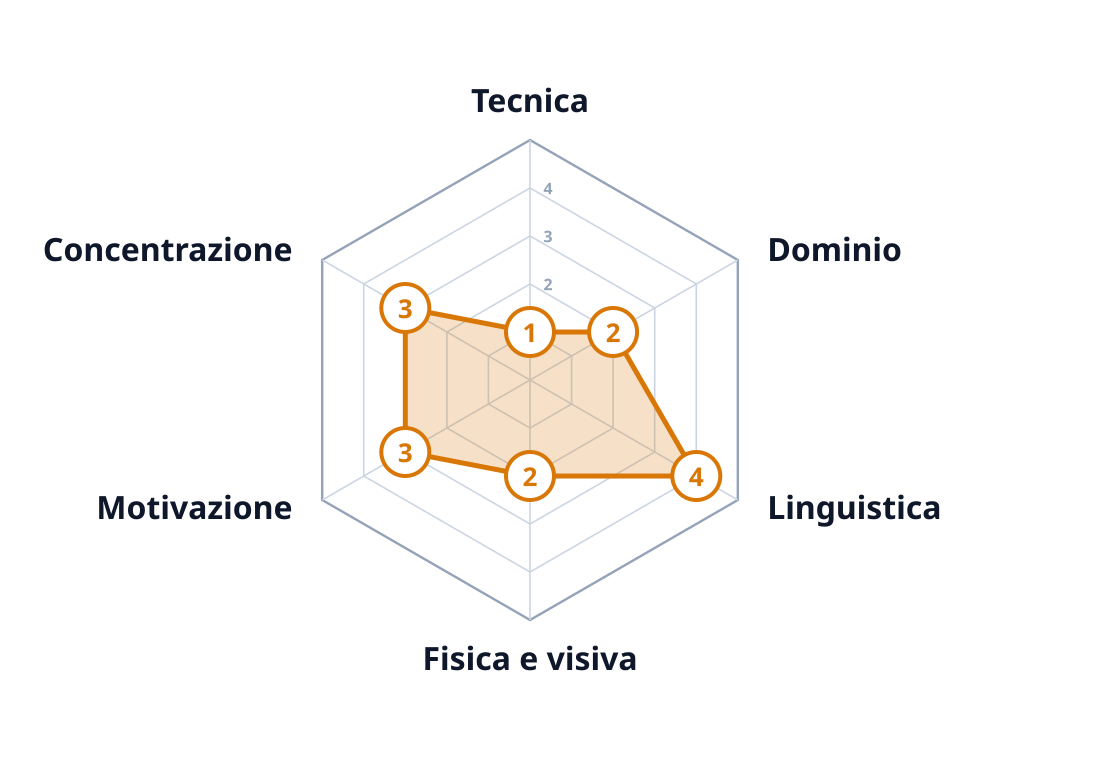
\includegraphics[width=0.88\linewidth]{assets/phase-b-persona-pina-skills.png}

\begin{longtable}{@{}p{0.24\linewidth}p{0.10\linewidth}p{0.59\linewidth}@{}}
\toprule
\textbf{Dimensione} & \textbf{1--5} & \textbf{Motivazione del punteggio} \\
\midrule
Tecnica & 1 & Non usa computer e dipende da aiuto per credenziali e flussi nuovi. \\
Dominio & 2 & Conosce visite ricorrenti, ma non canali e regimi amministrativi. \\
Linguistica & 4 & Comprende bene l'italiano comune; il lessico tecnico crea esitazione. \\
Fisica e visiva & 2 & Presbiopia e tremore rendono difficili testi e bersagli piccoli. \\
Motivazione & 3 & Vuole autonomia, ma l'ansia cresce dopo pochi tentativi falliti. \\
Concentrazione & 3 & Procede con cura; interruzioni ed errori riducono la continuità. \\
\bottomrule
\end{longtable}

\fieldheading{Scenario: la visita diabetologica di controllo}

Pina deve prenotare la visita semestrale. Recupera l'impegnativa, controlla
gli impegni sul calendario cartaceo e prova ER Salute. Non ricorda la password
SPID, confonde ``Prenota'' con ``Informazioni'' e non comprende un errore.
Dopo due tentativi chiama Elena durante una riunione. Il compito richiede
circa 10--15 minuti prima della richiesta di aiuto. Il successo consiste nel
comprendere il passo corrente, scegliere sede e data consapevolmente e
ricevere una conferma verificabile senza sostituzione da parte della figlia.
I rischi principali sono errore di selezione, frustrazione, abbandono e
rinuncia futura.

\fieldheading{Implicazioni di design}

\begin{itemize}
\item {[}P-01{]} L'autenticazione deve ridurre il carico di memoria e offrire recupero guidato; per attività solo consultive va evitata un'autenticazione ripetuta non necessaria.
\item {[}P-02{]} Azioni e bersagli devono essere grandi, distinti per forma, testo e icona, non soltanto per colore.
\item {[}P-03{]} Il linguaggio deve essere semplice e rassicurante, con conseguenze e conferme esplicite.
\item {[}U1-01{]} Il percorso per una visita ricorrente deve conservare il contesto e ridurre i passaggi senza decidere al posto dell'utente.
\item {[}U1-02{]} Prima dell'abbandono, un errore deve indicare causa, recupero e modalità di richiesta d'aiuto.
\end{itemize}

\cardsection{Documento 02b: Persona and Use Case card: personaggio secondario}

\personaphoto{Elena Ferretti}

\fieldheading{Identità, ruolo e segmento}

\begin{longtable}{@{}p{0.25\linewidth}p{0.69\linewidth}@{}}
\toprule
Nome e livello & Elena Ferretti --- personaggio secondario, caregiver di Pina \\
Segmento & Segmento B: caregiver familiare sempre reperibile a distanza, intermediaria \\
Profilo & 52 anni, impiegata amministrativa, vive a Bologna; famiglia, lavoro e assistenza alla madre \\
Dispositivi & PC e smartphone usati quotidianamente; elevata familiarità con servizi digitali \\
Vincoli & Poco tempo, interruzioni, carico emotivo e rischio di confondere profili o prenotazioni \\
\bottomrule
\end{longtable}

\begin{quote}
\emph{``Vorrei che mia madre potesse cavarsela da sola per le cose semplici, così mi preoccuperei solo per l'importante.''}

\small Citazione sintetica: ipotesi narrativa da sostituire o corroborare con
evidenze anonime delle interviste.
\end{quote}

\evidencestatus{Profilo provvisorio derivato dal Segmento B e dalle domande
B1--B6. La relazione con Pina esplicita il rapporto HPHP, ma frequenza e peso
dell'assistenza devono essere validati.}

\fieldheading{Comportamenti, esperienza e rete di aiuto}

Elena gestisce prenotazioni e disdette da remoto, spesso durante il lavoro.
Conosce CUPweb ed ER Salute, ma deve ricostruire dati, credenziali e intenzione
della madre a ogni richiesta. Accetta la delega solo se vede chiaramente per
chi sta agendo, che cosa cambierà e se Pina sarà informata. Il suo obiettivo è
ridurre le emergenze senza perdere la possibilità di intervenire nei casi
complessi; teme errori sul profilo sbagliato e notifiche insufficienti.

\fieldheading{Competenze e abilità (C\&A)}

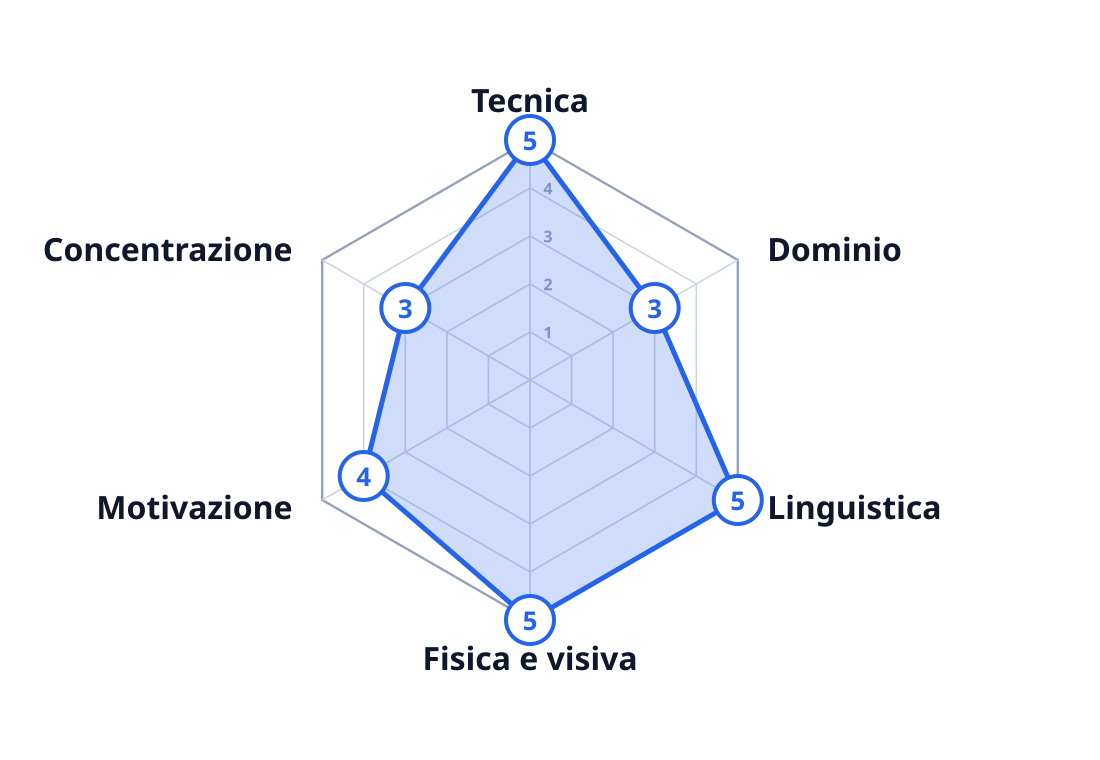
\includegraphics[width=0.88\linewidth]{assets/phase-b-persona-elena-skills.png}

\begin{longtable}{@{}p{0.24\linewidth}p{0.10\linewidth}p{0.59\linewidth}@{}}
\toprule
\textbf{Dimensione} & \textbf{1--5} & \textbf{Motivazione del punteggio} \\
\midrule
Tecnica & 5 & Usa quotidianamente PC, smartphone e servizi autenticati. \\
Dominio & 3 & Ha esperienza pratica, ma deve ricostruire prescrizioni e regimi. \\
Linguistica & 5 & Legge rapidamente anche testi amministrativi. \\
Fisica e visiva & 5 & Non emergono limitazioni rilevanti per il compito. \\
Motivazione & 4 & È motivata a proteggere Pina e a ridurre le interruzioni. \\
Concentrazione & 3 & Le richieste arrivano mentre lavora o gestisce la famiglia. \\
\bottomrule
\end{longtable}

\fieldheading{Scenario: la disdetta urgente dall'ufficio}

Durante il lavoro Elena riceve una chiamata da Pina: una visita va disdetta.
Deve identificare profilo e appuntamento corretti, controllare le conseguenze,
completare l'azione e rassicurare la madre in circa 5 minuti, prima di una
riunione. Il successo consiste in una disdetta verificabile, senza errore di
persona o appuntamento, con stato visibile a entrambe. Il rischio è che la
velocità spinga Elena a sostituirsi stabilmente a Pina.

\fieldheading{Implicazioni di design}

\begin{itemize}
\item {[}P-04{]} Il caregiver deve avere una visibilità chiara e proporzionata sulle prenotazioni autorizzate del familiare, con identità sempre evidente.
\item {[}P-05{]} La delega deve essere progressiva: Pina conserva le azioni semplici, Elena interviene nei casi complessi senza sorveglianza continua.
\item {[}U2-01{]} La disdetta deve richiedere pochi passaggi, distinguere appuntamenti simili e rendere esplicite le conseguenze.
\item {[}U2-02{]} Lo stato aggiornato e notifiche concordate devono ridurre telefonate di verifica e interventi d'emergenza.
\end{itemize}

\cardsection{Documento 02c: Persona and Use Case card: personaggio aggiuntivo}

\personaphoto{Renato Bellini}

\fieldheading{Identità, ruolo e segmento}

\begin{longtable}{@{}p{0.25\linewidth}p{0.69\linewidth}@{}}
\toprule
Nome e livello & Renato Bellini --- personaggio aggiuntivo di livello inferiore \\
Segmento & Segmento A: ``nuovo utente digitale'' 65--74, utente diretto moderatamente autonomo \\
Profilo & 70 anni, pensionato (ex assistente di biblioteca), vive a Forlì con la moglie; figlio adulto nelle vicinanze \\
Dispositivi & Tablet e smartphone; messaggistica, e-mail e SPID usato occasionalmente \\
Vincoli & Affaticamento visivo, rigidità delle mani, esitazione davanti a terminologia sanitaria o amministrativa ambigua \\
\bottomrule
\end{longtable}

\begin{quote}
\emph{``Se capisco cosa sto confermando, preferisco fare da solo e chiedere aiuto solo quando serve.''}

\small Citazione sintetica: ipotesi narrativa da sostituire o corroborare con
evidenze anonime delle interviste.
\end{quote}

\evidencestatus{Persona provvisoria costruita dal Segmento A e dalle domande
A1--A6. Serve come controllo del progetto, non come risultato già validato:
biografia, comportamenti, scenario e punteggi potranno cambiare dopo le
interviste.}

\fieldheading{Comportamenti, esperienza e rete di aiuto}

Renato prenota in autonomia quando riconosce il tipo di prestazione e il
regime; in alternativa telefona o chiede al figlio di verificare, non di
operare al suo posto. Ha già usato SPID e provato CUPweb/ER Salute, ma si
ferma davanti a etichette come ``SSN'', ``libera professione'' o costi non
immediatamente visibili. Teme una conferma onerosa o nella sede sbagliata.
Si sente autonomo se può leggere con calma, tornare indietro senza perdere le
scelte e verificare un riepilogo prima dell'invio. Descrive il proprio rapporto
con il digitale come positivo, purché il servizio non lo tratti da inesperto.

\fieldheading{Competenze e abilità (C\&A)}

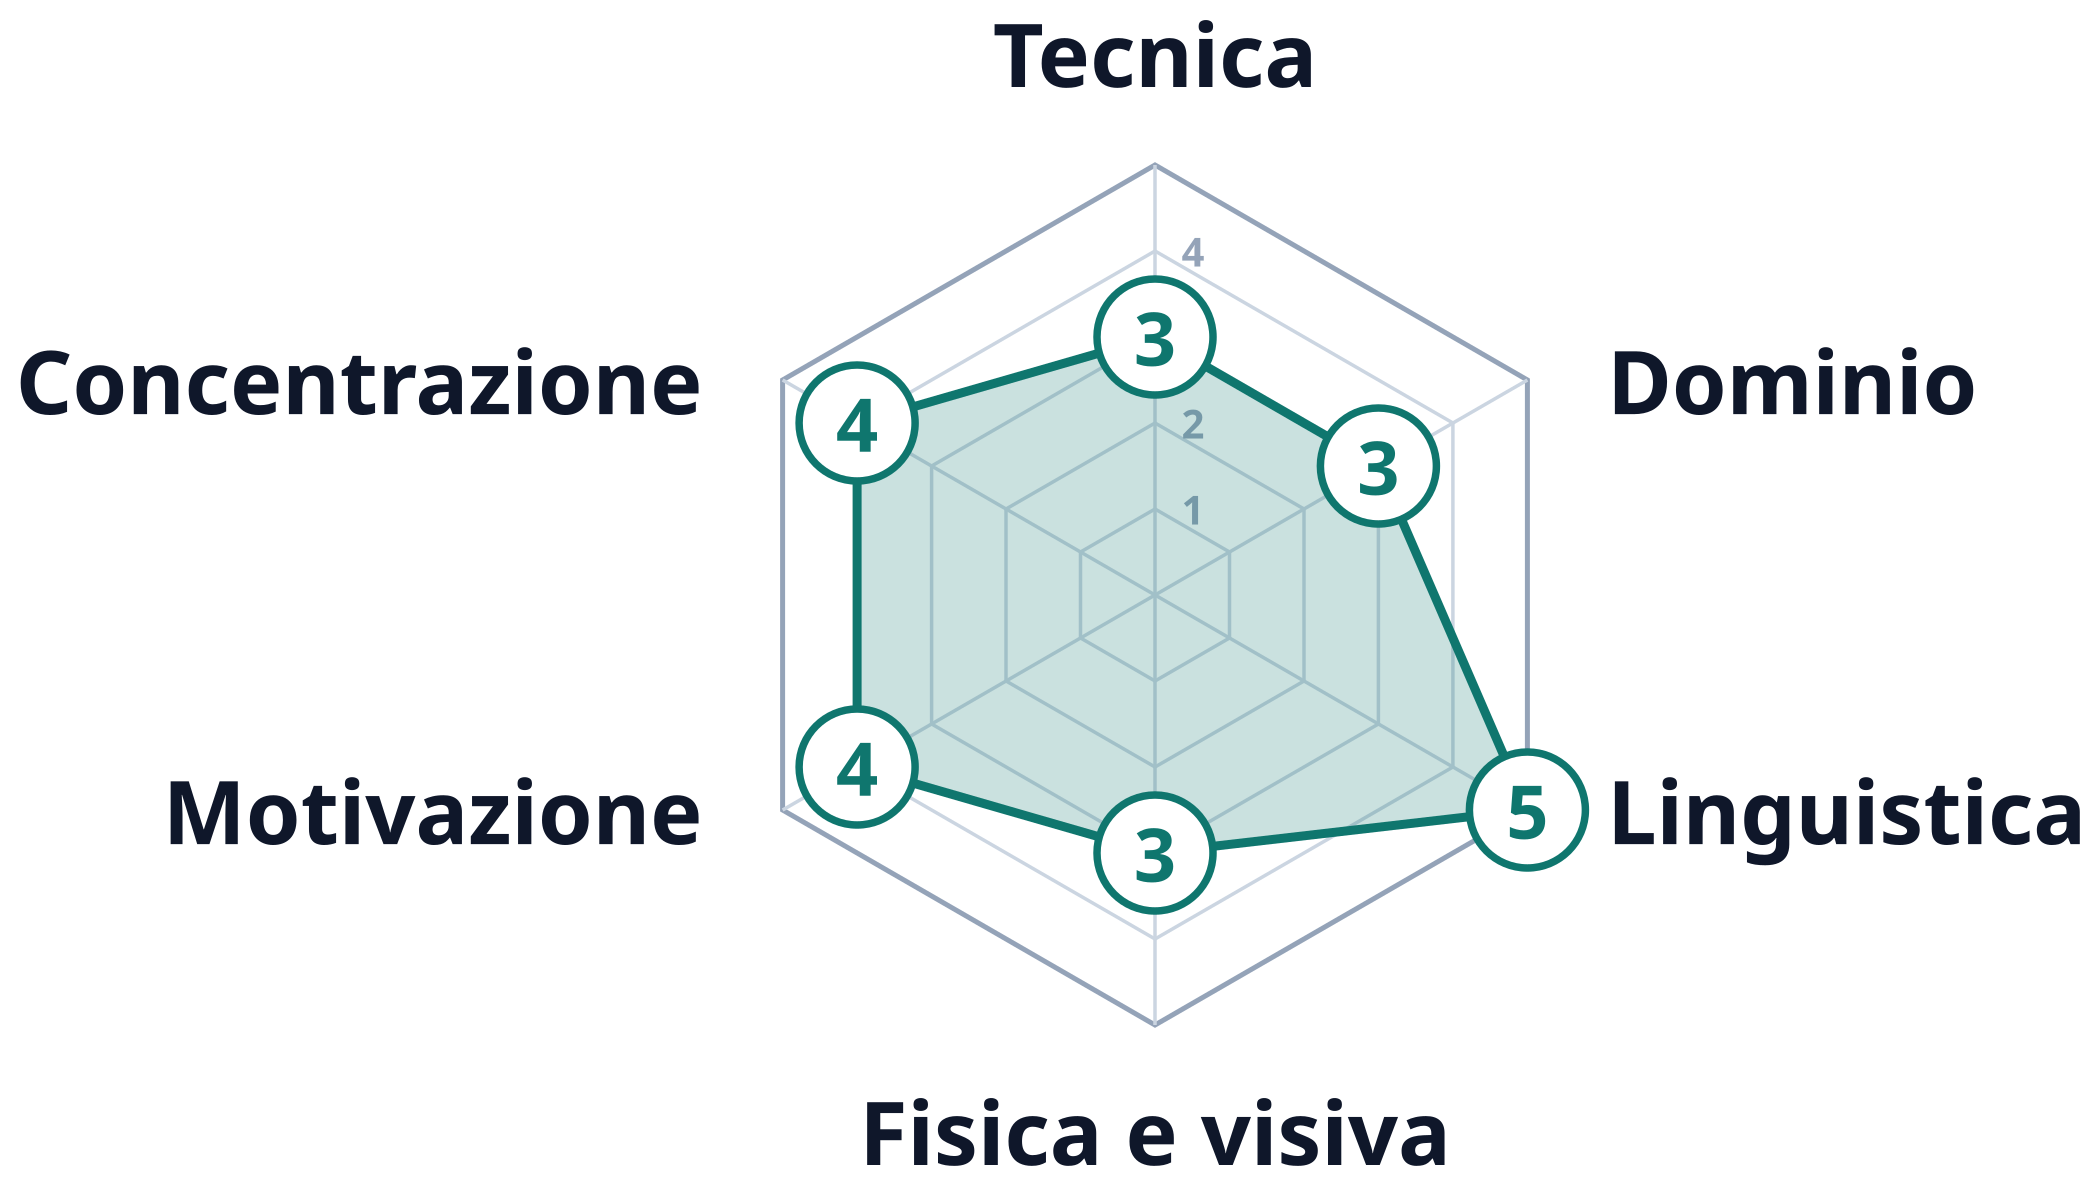
\includegraphics[width=0.88\linewidth]{assets/phase-b-persona-renato-skills.png}

\begin{longtable}{@{}p{0.24\linewidth}p{0.10\linewidth}p{0.59\linewidth}@{}}
\toprule
\textbf{Dimensione} & \textbf{1--5} & \textbf{Motivazione del punteggio} \\
\midrule
Tecnica & 3 & Usa servizi comuni e SPID, ma non automatizza procedure nuove. \\
Dominio & 3 & Conosce il percorso sanitario, non sempre regimi e conseguenze. \\
Linguistica & 5 & Legge e comprende bene; l'ambiguità terminologica è il limite. \\
Fisica e visiva & 3 & Affaticamento e rigidità richiedono buona leggibilità e bersagli ampi. \\
Motivazione & 4 & Preferisce operare da solo e considera l'aiuto una verifica mirata. \\
Concentrazione & 4 & Riesce a seguire il flusso se può fermarsi e riprendere senza perdere dati. \\
\bottomrule
\end{longtable}

\fieldheading{Scenario: il controllo oculistico senza chiamare il figlio}

Renato riceve l'impegnativa e prova a prenotare dal tablet. Confronta due
sedi, consulta il calendario e si ferma quando non distingue con certezza
SSN e libera professione. Vorrebbe verificare il significato senza perdere le
scelte già fatte. Stima di concludere in 8--10 minuti. Il successo consiste
nel prenotare sede, data e regime voluti, comprendere il costo e conservare
una conferma; chiedere una spiegazione non deve obbligarlo a cedere il compito
al figlio. I rischi sono affaticamento, scelta costosa e percezione di un
servizio paternalistico.

\fieldheading{Implicazioni di design}

\begin{itemize}
\item {[}P-06{]} Le spiegazioni devono essere progressive e facoltative: disponibili nel punto di dubbio, senza rallentare chi ha già compreso.
\item {[}P-07{]} Testo, spaziatura e bersagli devono restare leggibili e azionabili anche con affaticamento visivo e precisione ridotta.
\item {[}P-08{]} Regime, costo e conseguenze devono essere visibili in linguaggio rispettoso, senza semplificazioni paternalistiche.
\item {[}U3-01{]} Consultare una spiegazione, tornare indietro o chiedere aiuto non deve cancellare le scelte già effettuate.
\item {[}U3-02{]} Prima della conferma, un riepilogo deve mostrare prestazione, sede, data, regime e costo.
\end{itemize}

\cardsection{Documento 03: Cast card}

\fieldheading{Gerarchia, relazione e funzione nel cast}

\begin{enumerate}
\item \textbf{Pina --- protagonista.} Caso guida per accessibilità, fiducia e autonomia minima.
\item \textbf{Elena --- secondaria.} Caregiver a distanza collegata a Pina; rende visibile il conflitto tra assistenza e sostituzione.
\item \textbf{Renato --- aggiuntivo.} Controlla che le soluzioni per Pina non penalizzino efficienza, dignità e autonomia di un anziano più competente.
\end{enumerate}

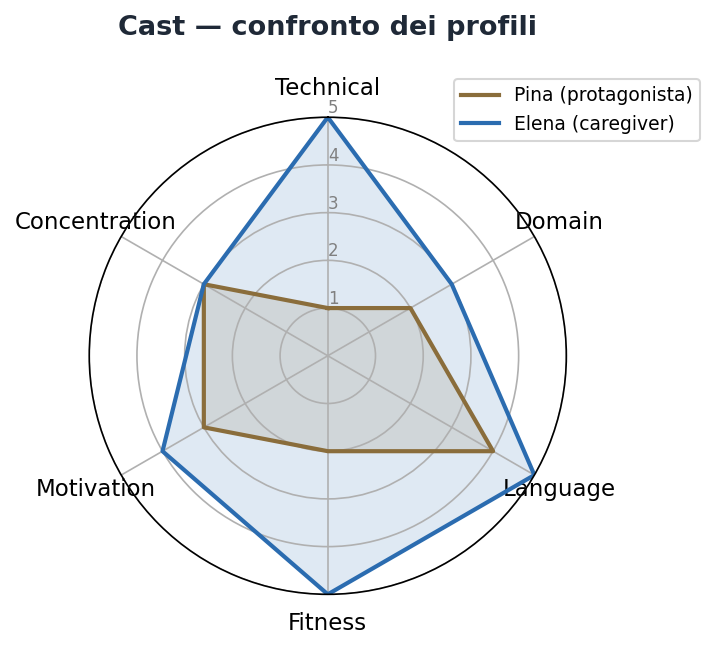
\includegraphics[width=\linewidth]{assets/phase-b-personas-comparison.png}

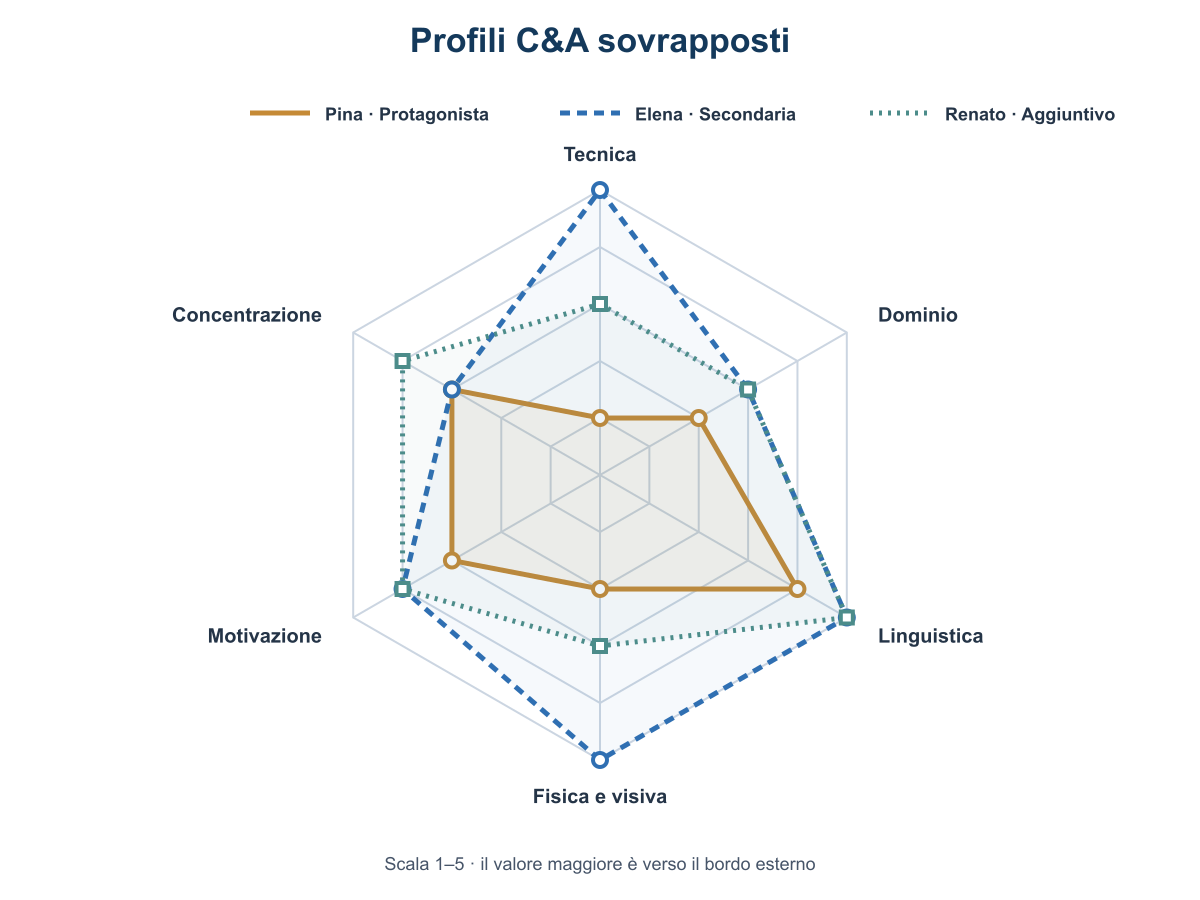
\includegraphics[width=0.90\linewidth]{assets/phase-b-personas-overlay.png}

Il workbook \texttt{phase-b-personas-and-cast.xlsx} contiene valori sorgente,
motivazioni, grafici radar editabili, matrice comparativa e schede scenario.
La heatmap e tutti i radar usano la scala diretta 1--5: il valore 1 è vicino
al centro, mentre il valore 5 raggiunge il bordo esterno. Il radar sovrapposto
permette di confrontare il profilo complessivo delle tre persone.

\fieldheading{Motivazione della selezione e alternative scartate}

Pina ed Elena coprono i due segmenti prioritari e la relazione HPHP centrale.
Renato introduce una variazione interna al Segmento A e verifica il bilanciamento
tra semplicità ed efficienza. Sono state rinviate: una caregiver convivente con
competenza media, perché aggiunge poca variabilità rispetto a Elena; una figura
sanitaria o di farmacia, perché esterna ai segmenti intervistati; una persona
completamente dipendente, perché sarebbe un caso limite artificiale senza
evidenze sufficienti. Anche gli scenari di sola consultazione e di modifica
anagrafica sono rinviati perché meno rappresentativi del problema di
prenotazione e assistenza emerso in Fase A.

\fieldheading{Matrice persona -- domande di Fase A -- validazione}

\begin{longtable}{@{}p{0.15\linewidth}p{0.31\linewidth}p{0.28\linewidth}p{0.18\linewidth}@{}}
\toprule
\textbf{Persona} & \textbf{Elemento} & \textbf{Domanda/evidenza Fase A} & \textbf{Stato} \\
\midrule
Pina & Prenotazione attuale, tentativi digitali, aiuto, paure e autonomia & Segmento A, domande A1--A6 & Ipotesi da validare \\
Pina & Vincoli visivi e motori; punteggi C\&A & Domande A4--A6; osservazione futura & Ipotesi da validare \\
Elena & Carico, urgenza e gestione da remoto & Segmento B, domande B1--B2 e B6 & Ipotesi da validare \\
Elena & Delega, fiducia, visibilità e controllo & Domande B3--B5 & Ipotesi da validare \\
Renato & Canali attuali e tentativi CUPweb/ER Salute & Domande A1--A2 & Ipotesi da validare \\
Renato & Quando chiede aiuto e che cosa teme & Domande A3--A4 & Ipotesi da validare \\
Renato & Condizioni di autonomia e rapporto con il digitale & Domande A5--A6 & Ipotesi da validare \\
\bottomrule
\end{longtable}

\fieldheading{Conflitti progettuali}

\begin{itemize}
\item Una guida sempre visibile sostiene Pina ma può rallentare Renato: servono spiegazioni progressive e richiudibili.
\item Le scorciatoie utili a Elena non devono nascondere identità, stato o conseguenze dell'azione.
\item La supervisione rassicura il caregiver, ma può diventare sorveglianza o sostituzione dell'utente diretto.
\item Controlli grandi e spaziati devono convivere con una densità informativa sufficiente per chi opera rapidamente.
\end{itemize}

\fieldheading{Requisiti cumulativi del cast}

\begin{itemize}
\item {[}C-01{]} (= P-01+P-02+P-03) Il servizio deve essere utilizzabile con competenza tecnica minima, azioni visibili e tono rassicurante.
\item {[}C-02{]} (= P-04+P-05) Visibilità e delega devono sostenere una supervisione leggera, autorizzata e non sostitutiva.
\item {[}C-03{]} (= U1-01+U2-01) Prenotazione ricorrente e disdetta devono ridurre passaggi e ambiguità mantenendo il controllo dell'utente.
\item {[}C-04{]} (= U1-02+U2-02) Errori e cambi di stato devono offrire recupero comprensibile e notifiche concordate.
\item {[}C-05{]} (= P-03+P-04) Identità, oggetto e conseguenze dell'azione devono essere espliciti per utente diretto e caregiver.
\item {[}C-06{]} (= P-06+P-08) Spiegazioni progressive devono chiarire termini, regime, costo e conseguenze senza infantilizzare.
\item {[}C-07{]} (= P-02+P-07) Gerarchia, leggibilità, spaziatura e dimensione dei bersagli devono supportare vincoli visivi e motori.
\item {[}C-08{]} (= U3-01+U3-02) Il sistema deve conservare le scelte durante consultazione e aiuto, quindi mostrare un riepilogo completo prima della conferma.
\end{itemize}

% !TEX root = ../hphp-project-report.tex
\chapter{Fase C: Design Proposal}

\section{Modello di design e strategia metodologica}

\subsection{Adozione del modello di design}

Per guidare la transizione dalle evidenze empiriche ed etnografiche delle Fasi A e B alla proposta operativa di riprogettazione, il team ha adottato formalmente il modello concettuale a strati di \textbf{Jesse James Garrett} (\emph{The Elements of User Experience}), integrato con i principi del \textbf{Goal-Directed Design} di \textbf{Alan Cooper} (\emph{About Face}) e il ciclo iterativo dello standard \textbf{ISO 9241-210} (\emph{Human-Centred Design for Interactive Systems}).

Il modello di Garrett struttura il processo progettuale su cinque livelli progressivi di decisione, dal piano astratto a quello tangibile:
\begin{enumerate}
\item \textbf{Strategy Plane:} definisce gli obiettivi organizzativi della sanità regionale (riduzione delle liste d\textquotesingle attesa, abbattimento del tasso di abbandono digitale, inclusione delle fasce fragili) e i bisogni profondi emersi dai modelli mentali delle quattro personas (autonomia protetta per Pina, efficienza a basso attrito per Elena, trasparenza e controllo per Renato, mediazione e flessibilità per Amina).
\item \textbf{Scope Plane:} delimita le funzionalità offerte e i requisiti informativi, formalizzando la coesistenza di due binari operativi complementari: la \textbf{Modalità Co-Pilota} (assistenza collaborativa in tempo reale) e la \textbf{Modalità Delega Piena} (gestione asincrona per conto terzi).
\item \textbf{Structure Plane:} definisce l\textquotesingle Information Architecture (organizzazione dei contenuti e sistema di etichettatura per compiti) e l\textquotesingle Interaction Design (flussi operativi, gestione del feedback, tolleranza agli errori) attraverso diagrammi di struttura formali (\emph{Structure Blueprints}).
\item \textbf{Skeleton Plane:} definisce l\textquotesingle arrangiamento visivo, la gerarchia delle informazioni desktop e i componenti di navigazione attraverso la suite di wireframe per computer (Versione 0).
\item \textbf{Surface Plane:} definisce il linguaggio visivo, i contrasti cromatici e il microcopy in linguaggio naturale (\emph{Plain Language}).
\end{enumerate}

\subsection{Integrazione degli approcci Top-down e Bottom-up}

L\textquotesingle architettura del sistema è stata concepita mediante una sintesi metodologica bidirezionale:
\begin{itemize}
\item \textbf{Approccio Top-down (dagli obiettivi alla strategia):} parte dai macro-obiettivi di servizio pubblico della Regione Emilia-Romagna e dai profili comportamentali del cast di personas. Questo approccio guida la suddivisione delle funzionalità nelle cinque macro-aree orientate ai compiti del cittadino e struttura il principio di \emph{empowerment non sostitutivo}: l\textquotesingle anziano mantiene la titolarità dell\textquotesingle azione sulla propria postazione PC, mentre il caregiver interviene come supporto visivo e rassicurativo a distanza.
\item \textbf{Approccio Bottom-up (dalle parti al sistema):} parte dall\textquotesingle inventario atomico dei dati e dei documenti sanitari reali (la ricetta dematerializzata con codice NRE a 15 caratteri, le disponibilità orarie dei calendari CUP delle singole AUSL, gli avvisi di pagamento pagoPA, le deleghe formali registrate nel Fascicolo Sanitario Elettronico). Il sistema aggrega queste componenti frammentate e le ricompone in un flusso lineare su layout desktop, delegando all\textquotesingle infrastruttura informatica il routing tra i diversi database e sollevando l\textquotesingle utente dall\textquotesingle onere della classificazione manuale.
\end{itemize}

\subsection{Importazione e priorità dei requisiti di design}

La proposta di design recepisce integralmente e rende operativi i requisiti numerati consolidati nelle conclusioni della Fase A (\texttt{REQ-01}...\texttt{REQ-09}) e nelle schede delle personas e del cast della Fase B (\texttt{P-01}...\texttt{P-11}, \texttt{U1}...\texttt{U4}, \texttt{C-01}...\texttt{C-12}).

\begin{center}
\small
\begin{tabular}{@{}llcp{0.48\linewidth}@{}}
\toprule
\textbf{Requisito} & \textbf{Origine} & \textbf{Priorità} & \textbf{Decisione Progettuale Chiave in Fase C} \\
\midrule
\textbf{REQ-01} & ID-01, P-01 & Alta & Accesso iniziale con autenticazione all\textquotesingle ingresso del portale: primo accesso o rinnovo tramite SPID/CIE con impostazione contestuale di un PIN personale a 30 giorni (modello INPS), seguito da accesso rapido quotidiano tramite solo PIN dal PC domestico; navigazione interna interamente profilata e priva di interruzioni durante la prenotazione. \\
\textbf{REQ-02} & ID-02, R-02 & Alta & Unificazione visiva e sistemica dei touchpoint sotto un\textquotesingle unica interfaccia HPHP coerente. \\
\textbf{REQ-03} & ID-03, ID-04, P-08 & Media & Gerarchia visiva ad alto contrasto, Plain Language, trasparenza tariffe SSN vs Libera Professione. \\
\textbf{REQ-04} & ID-05, ID-08, P-03 & Alta & Flusso guidato a step, isolamento dei comandi distruttivi, dicitura esplicita di reversibilità/modifica. \\
\textbf{REQ-05} & ID-06, R-05 & Media & Struttura semantica desktop chiara, pulsanti ad alta salienza visiva, compatibilità screen reader. \\
\textbf{REQ-06} & ID-10, P-04, P-05 & Alta & Modalità Co-Pilota (guida in tempo reale non espropriativa) e Delega Piena asincrona tracciata. \\
\textbf{REQ-07} & ID-09, P-10, U4-02 & Alta & Riepilogo dettagliato anti-duplicati con stampa A4 ad alta leggibilità, condivisione WhatsApp, SMS e calendario. \\
\textbf{REQ-08} & ID-11, P-11, U4-01 & Media & Resilienza a standby e interruzioni: congelamento stato task per 24 ore e ripresa assistita in farmacia/CUP. \\
\textbf{REQ-09} & ID-12, R-09 & Media & Canale di assistenza scritto/asincrono contestuale affiancato alla rete territoriale delle farmacie. \\
\bottomrule
\end{tabular}
\end{center}

\subsection{Principi di tono, voce e messaggio}

Poiché il tono e il registro linguistico influenzano direttamente la motivazione e la fiducia degli utenti più fragili, sono state definite tre linee guida comunicative vincolanti per tutte le schermate:
\begin{itemize}
\item \textbf{Plain Language contro la burocrazia tecnica:} eliminazione totale delle diciture ministeriali aride in ALL CAPS (riscontrate nell\textquotesingle assessment di CUPweb) e delle sigle opache. I termini tecnici necessari (es. NRE, intramoenia, impegnativa) sono sempre affiancati da glosse esplicative in linguaggio comune ed esempi visivi contestuali (\texttt{REQ-03}, \texttt{P-09}, \texttt{C-09}).
\item \textbf{Rassicurazione attiva e reversibilità garantita:} superamento dell\textquotesingle ansia da errore irreversibile (\texttt{ID-08}, \texttt{P-03}). L\textquotesingle interfaccia esplicita chiaramente prima di ogni azione critica: \emph{``Non ti preoccupare: potrai modificare o disdire gratuitamente questo appuntamento in qualsiasi momento fino a 48 ore prima della visita''}. I pulsanti di cancellazione sono cromaticamente e spazialmente separati dai pulsanti di conferma (\texttt{C-07}).
\item \textbf{Rispetto e non infantilizzazione:} il tono di voce è accogliente, chiaro e incoraggiante, ma mantiene la serietà di un servizio istituzionale di salute pubblica. Non adotta toni paternalistici o sminuenti, preservando la dignità e l\textquotesingle autonomia dell\textquotesingle adulto anziano (\texttt{P-08}, \texttt{C-06}).
\end{itemize}

\subsection{Delimitazione dello scope e strategia d\textquotesingle accesso Desktop-First}

Il progetto HPHP si concentra formalmente sulla riprogettazione dell\textquotesingle esperienza utente di \textbf{CUPweb come portale web per personal computer (Desktop PC)}. 

Nell\textquotesingle ecosistema della sanità digitale della Regione Emilia-Romagna, l\textquotesingle accesso in mobilità tramite smartphone è affidato all\textquotesingle applicazione nativa per dispositivi mobili \textbf{ER Salute}. Tale applicazione risponde a requisiti, pattern d\textquotesingle interazione e contesti d\textquotesingle uso marcatamente distinti, e si colloca formalmente al di fuori del dominio e dell\textquotesingle obiettivo didattico del presente progetto. Pertanto, l\textquotesingle ottimizzazione specifica per schermi smartphone non costituisce l\textquotesingle oggetto di questo redesign.

Coerentemente con i moderni standard di ingegneria web, l\textquotesingle interfaccia adotta comunque un\textquotesingle architettura responsive fluida per garantire che il layout mantenga integrità strutturale qualora aperto su schermi di dimensioni ridotte. Tuttavia, **tutte le decisioni di Information Architecture, gli Structure Blueprints e la suite completa dei wireframe sono rigorosamente progettati e ottimizzati per l\textquotesingle ambiente Desktop PC** (risoluzione di riferimento 1280$\times$800 / 1440$\times$900\,px). 

Questa focalizzazione risponde direttamente ai contesti operativi reali documentati nelle personas di Fase B:
\begin{itemize}
\item \textbf{Ergonomia d\textquotesingle uso per l\textquotesingle utente anziano (Pina, Renato):} l\textquotesingle interazione su grande schermo elimina la claustrofobia visiva del display mobile, consente l\textquotesingle impiego di caratteri tipografici ampi e contrastati, riduce l\textquotesingle errore da tocco accidentale grazie alla stabilità del mouse e permette di avere sott\textquotesingle occhio contemporaneamente la ricetta cartacea appoggiata sulla scrivania e i campi a video.
\item \textbf{Densità e trasparenza comparativa:} l\textquotesingle ampiezza dello schermo desktop consente di affiancare in un\textquotesingle unica vista tabelle comparative ricche (canale pubblico SSN vs libera professione ALPI) e mappe territoriali integrate all\textquotesingle elenco delle strutture sanitarie, senza costringere l\textquotesingle utente a complessi cambi di schermata.
\item \textbf{Postazione di lavoro del caregiver (Elena, Amina):} la figlia lavoratrice Elena opera frequentemente dal computer dell\textquotesingle ufficio o da casa, dove una dashboard desktop a tutta larghezza consente una gestione efficiente, sicura e multi-profilo della salute dei genitori.
\end{itemize}

\cardsection{Documento 02: Information Architecture card}

\subsection{Ruolo e necessità dell\textquotesingle Information Architecture}

Una fase di riprogettazione specifica dell\textquotesingle Information Architecture è risultata indispensabile e propedeutica a qualsiasi scelta di interfaccia grafica. L\textquotesingle analisi di Fase A ha infatti dimostrato che la barriera primaria di usabilità dell\textquotesingle attuale sistema non risiede soltanto nell\textquotesingle estetica visiva, ma nella frammentazione strutturale dell\textquotesingle informazione sanitaria regionale, suddivisa su tre piattaforme autonome e scollegate: CUPweb per la prenotazione, il Fascicolo Sanitario Elettronico (FSE) per ricette e referti, e pagoPA / Pagonlinesanità per il pagamento del ticket.

L\textquotesingle architettura attuale riflette i confini burocratici dei fornitori IT e dei database delle singole AUSL, costringendo il cittadino a conoscere a priori l\textquotesingle organigramma della Pubblica Amministrazione. Ridisegnare le schermate senza ristrutturare a monte l\textquotesingle Information Architecture avrebbe lasciato intatto il disorientamento cognitivo, la ridondanza e il timore di abbandono documentati nei test empirici (\texttt{ID-02}, \texttt{R-02}, \texttt{REQ-02}).

\subsection{Approccio architetturale: Top-down vs. Bottom-up}

L\textquotesingle architettura dell\textquotesingle informazione adotta una sintesi integrata tra due approcci complementari:
\begin{itemize}
\item \textbf{Top-down:} definisce la gerarchia delle macro-categorie di primo livello a partire dai modelli mentali degli utenti emersi dalle personas (i compiti della vita reale: prenotare, consultare gli appuntamenti, visualizzare le ricette, delegare la cura, chiedere supporto).
\item \textbf{Bottom-up:} cataloga e organizza i singoli oggetti informativi minimi (NRE, quesito diagnostico, branca specialistica, codice fiscale, quietanza di pagamento, fermate bus) garantendo che ciascun dato sia collocato nel punto esatto in cui l\textquotesingle utente se lo aspetta e che le etichette utilizzino termini d\textquotesingle uso comune.
\end{itemize}

\subsection{Razionale della discontinuità rispetto al tool esistente}

La scelta architetturale segna una netta discontinuità rispetto all\textquotesingle impostazione di CUPweb. Il sistema esistente adotta un modello organizzativo rigidamente orientato ai silos di backend: la home page costringe l\textquotesingle utente a scegliere tra quattro percorsi amministrativi mutuamente esclusivi prima ancora di aver inserito qualsiasi dato:
\begin{enumerate}
\item \emph{Prenota ricette di specialistica};
\item \emph{Prenota ricette esami di laboratorio};
\item \emph{Prenota un Accesso all\textquotesingle Anagrafe Sanitaria o Sanità Pubblica};
\item \emph{Prenota prestazioni di medicina dello sport}.
\end{enumerate}
Questo modello scarica sull\textquotesingle anziano fragile l\textquotesingle onere di comprendere la tassonomia sanitaria regionale (es. sapere se un controllo diabetologico ricada nella specialistica o nella sanità pubblica), generando blocchi decisionali immediati (Pina) e schermate di errore sterili.

Nel redesign HPHP l\textquotesingle architettura è integralmente **orientata ai compiti dell\textquotesingle utente (Task-Driven)**. Il portale desktop offre un unico punto d\textquotesingle accesso intuitivo (\emph{``Prenota una visita o un esame''}): il motore di sistema riconosce automaticamente dal codice ricetta (NRE) o dalle parole chiave se la prestazione sia una visita specialistica, un esame ematochimico o una vaccinazione, smistando la richiesta alle agende appropriate in modo invisibile all\textquotesingle utente.

\subsection{Decisioni sull\textquotesingle organizzazione e sistema di etichettatura}

La navigazione desktop di primo livello si articola in **cinque macro-aree di navigazione globale**, formulate in linguaggio naturale (\emph{Plain Language}) e orientate all\textquotesingle azione:
\begin{enumerate}
\item \textbf{``Prenota una visita o esame'':} punto di ingresso unico e unificato. Elimina la frammentazione burocratica accogliendo l\textquotesingle utente con un bivio trasparente tra ricetta medica (NRE) e prestazioni ad accesso libero/private.
\item \textbf{``I miei appuntamenti'':} cruscotto unico desktop a tabella per visualizzare, consultare dettagli, spostare o disdire tutte le prestazioni future e lo storico pregresso, unificando le agende di tutte le AUSL regionali.
\item \textbf{``Le mie prescrizioni'':} archivio sincronizzato delle ricette dematerializzate prescritte dal medico di medicina generale, con indicazione visiva dello stato (da prenotare, già prenotata, scaduta).
\item \textbf{``Chi assisto'':} area dedicata alla gestione della relazione tra caregiver e assistito (\texttt{P-04}, \texttt{P-05}, \texttt{C-02}, \texttt{REQ-06}), con gestione delle deleghe legali FSE e switch profilo per operare con trasparenza.
\item \textbf{``Serve aiuto?'':} touchpoint di supporto sempre visibile nella barra globale, con FAQ visuali in linguaggio semplice, guida contestuale alla ricetta cartacea e strumento di salvataggio sessione per il completamento in farmacia o allo sportello CUP (\texttt{REQ-08}, \texttt{REQ-09}).
\end{enumerate}

\subsection{Schema dei metadati e modello concettuale}

Rispetto alla gestione tabellare grezza e isolata di CUPweb, l\textquotesingle architettura informativa arricchisce i dati sanitari con una semantica esplicita orientata all\textquotesingle accessibilità logistica, alla trasparenza economica e alla co-gestione familiare.

\begin{center}
\small
\begin{tabular}{@{}
  >{\raggedright\arraybackslash}p{0.24\linewidth}
  >{\raggedright\arraybackslash}p{0.52\linewidth}
  >{\raggedright\arraybackslash}p{0.18\linewidth}@{}}
\toprule
\textbf{Campo di Metadato} & \textbf{Ruolo Funzionale nel Portale Desktop} & \textbf{Requisiti Tracciati} \\
\midrule
\textbf{Distanza km e fermate TPL} & Calcolo automatico della vicinanza da casa; indicazione linee autobus con fermata a meno di 200\,m; ordinamento predefinito per prossimità territoriale. & REQ-03, U1-01, P-08 \\
\midrule
\textbf{Regime erogativo (SSN vs ALPI)} & Separazione trasparente tra canale pubblico e Libera Professione; visualizzazione preventiva del costo effettivo in euro e prima data utile in colonne affiancate. & REQ-03, P-08, ID-03 \\
\midrule
\textbf{Livello di identificazione} & Autenticazione preliminare all\textquotesingle ingresso del portale (SPID/CIE al primo accesso $\rightarrow$ impostazione PIN personale a 30 giorni stile INPS $\rightarrow$ accessi rapidi successivi con solo PIN); l\textquotesingle intera navigazione e prenotazione avvengono in contesto già identificato e profilato. & REQ-01, P-01, C-01 \\
\midrule
\textbf{PIN personale semplificato (30\,gg)} & Codice numerico a 4--5 cifre scelto direttamente dall\textquotesingle utente dopo il login SPID/CIE, richiesto nella schermata d\textquotesingle ingresso del portale per i successivi 30 giorni per consentire all\textquotesingle anziano di entrare rapidamente dal PC personale bypassando SPID e OTP. & REQ-01, P-01, REQ-08 \\
\midrule
\textbf{Profilo e ruolo di delega} & Distinzione tra paziente titolare e soggetto operatore; abilitazione del banner persistente colorato in testata; tracciamento delle autorizzazioni legali di delega FSE. & REQ-06, P-04, C-05 \\
\midrule
\textbf{Stato sessione Co-Pilota} & Segnalazione WebSocket attiva tra assistito e caregiver; sincronizzazione del puntatore visivo desktop e micro-canale audio di rassicurazione. & REQ-07, REQ-04, C-07 \\
\midrule
\textbf{Token sessione (24h)} & Generazione di un codice numerico univoco temporaneo per congelare lo stato del form in caso di stallo, consentendo la ripresa assistita in farmacia o al CUP fisico. & REQ-08, ID-11, C-11 \\
\midrule
\textbf{Stato prescrizione NRE} & Interrogazione del Sistema Tessera Sanitaria per distinguere ricette prenotabili, già utilizzate o scadute; alimentazione delle scorciatoie per patologie croniche. & REQ-02, P-09, U1-01 \\
\midrule
\textbf{Timer ripensamento (10 min)} & Applicazione delle regole regionali di preavviso (2 giorni lavorativi); finestra di sicurezza post-disdetta con banner persistente per ripristinare il posto con un click. & REQ-05, ID-08, C-03 \\
\bottomrule
\end{tabular}
\end{center}

\subsection{Progettazione del sistema di navigazione Desktop}

Il sistema di navigazione per computer desktop adotta una **struttura gerarchica lineare, ariosa e trasparente**:
\begin{itemize}
\item \textbf{Gate d\textquotesingle Ingresso Desktop (Livello 0):} schermata preliminare che accoglie l\textquotesingle utente all\textquotesingle apertura del portale richiedendo l\textquotesingle identificazione immediata. Presenta due canali visuali distinti ad alto contrasto: l\textquotesingle \textbf{Accesso Rapido con PIN Personale a 30 giorni} (tastierino a 4--5 cifre per gli utenti abituali sul PC domestico, che bypassa SPID ed entra istantaneamente) e l\textquotesingle \textbf{Accesso con SPID o CIE} (per il primo accesso, per dispositivi nuovi o dopo la scadenza dei 30 giorni, con contestuale invito a impostare il proprio PIN personale).
\item \textbf{Header Istituzionale e Navigazione Globale (Livello 1):} testata superiore persistente visibile in tutte le pagine interne autenticate, contenente il logo istituzionale del Servizio Sanitario Regionale, i controlli di accessibilità visiva per l\textquotesingle ingrandimento immediato dei caratteri (\texttt{A / A+ / A++}), l\textquotesingle indicatore del profilo utente autenticato (nome del cittadino, es. \emph{Giuseppina Ferretti}, stato dell\textquotesingle accesso rapido attivo per 30 giorni e pulsante di disconnessione sicura) e la barra orizzontale con le cinque macro-sezioni primarie.
\item \textbf{Breadcrumb e Stepper Orizzontale a Step (Livelli 2 e 3):} nei percorsi operativi guidati (wizard di prenotazione), l\textquotesingle avanzamento è scandito da uno stepper orizzontale superiore con numerazione ed etichette chiare (\emph{1. Tipo prestazione $\rightarrow$ 2. Ricetta/Dati $\rightarrow$ 3. Sede e Data $\rightarrow$ 4. Riepilogo}). È sempre presente un comando esplicito di ritorno (\emph{``$\leftarrow$ Torna al passaggio precedente''}) che preserva i filtri impostati senza azzerare i dati (\texttt{U3-01}).
\item \textbf{Banner di Contesto Caregiver Desktop:} quando il caregiver opera in modalità delegata per conto del familiare, la testata visualizza una barra arancione persistente a tutta larghezza (\emph{``Stai operando per conto di: Giuseppina Ferretti - Codice Fiscale: FRRGPP...''}), azzerando il rischio di confondere i profili (\texttt{P-04}, \texttt{C-05}).
\end{itemize}

\subsection{Sintesi delle componenti di Information Architecture}

Coerentemente con la tassonomia dell\textquotesingle Information Architecture di Rosenfeld e Morville (2002), le componenti del sistema si articolano in quattro categorie:

\subsubsection{Browsing Aids (Supporti alla navigazione)}
\begin{itemize}
\item \textbf{Widget ``Prossimo appuntamento'':} posizionato nel cruscotto della home page, evidenzia con caratteri grandi data, orario, sede e specialità della visita imminente, con conto alla rovescia rassicurante e tasto diretto per le indicazioni stradali o la preparazione alla visita.
\item \textbf{Scorciatoia ``Prenota di nuovo'':} per pazienti con patologie croniche o controlli periodici (Pina per il diabete, Renato per l\textquotesingle oculistica), propone una scorciatoia che pre-imposta la prestazione e il centro ospedaliero abituale.
\item \textbf{Badge Caregiver Collegato:} notifica visiva nella home page che indica lo stato del familiare di fiducia (\emph{``Tua figlia Elena è collegata''}), accrescendo il senso di protezione dell\textquotesingle anziano.
\end{itemize}

\subsubsection{Search Aids (Supporti alla ricerca)}
\begin{itemize}
\item \textbf{Ricerca semantica a tolleranza ortografica:} la barra di ricerca testuale desktop non richiede codici ministeriali o diciture esatte in maiuscolo; digitando termini d\textquotesingle uso comune (es. \emph{``controllo vista''}, \emph{``esami sangue''}, \emph{``vaccino influenza''}) il sistema suggerisce istantaneamente le prestazioni mediche pertinenti con brevi spiegazioni.
\item \textbf{Filtri strutturati a pulsanti visivi (Chips):} anziché menu a tendina densi e a comparsa rapida, i filtri di selezione (fascia oraria mattina/pomeriggio, raggio kilometrico entro 5/10/20\,km, regime pubblico/privato) sono pulsanti desktop stabili attivabili con un click del mouse.
\end{itemize}

\subsubsection{Contents and Tasks (Contenuti e gerarchia dei compiti)}
\begin{itemize}
\item \textbf{Compito Primario:} ricercare, comparare e fissare un appuntamento sanitario su schermo ampio, in piena autonomia o con il supporto del co-pilota familiare.
\item \textbf{Compito Secondario (Gestione):} verificare gli appuntamenti pianificati, disdire tempestivamente liberando il posto per altri cittadini o riprogrammare la data senza penalità economiche.
\item \textbf{Compito di Assistenza e Cura:} monitorare lo stato di salute dei familiari anziani, verificare la validità delle ricette e concordare le scelte sanitarie a distanza.
\item \textbf{Contenuti informativi periferici:} normative, privacy e regolamenti aziendali non competono con il flusso operativo principale, rimanendo consultabili nell\textquotesingle area \emph{``Serve aiuto?''} o richiamabili tramite schede informative contestuali.
\end{itemize}

\subsubsection{Invisible Components (Componenti invisibili di supporto)}
\begin{itemize}
\item \textbf{Session \& State Persistence Engine:} gestore locale della sessione che previene la scadenza improvvisa per inattività durante pause di riflessione o consultazione di documenti cartacei, preservando lo stato del form per 24 ore (\texttt{REQ-08}, \texttt{ID-11}) e gestendo in sicurezza il PIN personale a 30 giorni scelto direttamente dall\textquotesingle utente (ispirato al modello INPS per gli utenti anziani), riducendo la barriera dell\textquotesingle autenticazione a due fattori ripetuta nei successivi accessi dal computer personale.
\item \textbf{Real-Time Co-Browsing Signaling Gateway:} middleware basato su protocolli WebSocket/WebRTC che sincronizza la posizione del puntatore visivo tra il computer dell\textquotesingle assistito e quello del caregiver durante la Modalità Co-Pilota, senza trasmissione di flussi video pesanti.
\item \textbf{Regional Interoperability Bus:} bus di integrazione che interroga in parallelo il Sistema Tessera Sanitaria (validità NRE), i server CUP regionali (disponibilità agende), il Fascicolo Sanitario Elettronico (storico clinico) e il gateway pagoPA.
\item \textbf{Bilateral Notification Dispatcher:} motore multicanale che invia conferme e promemoria sincronizzati su SMS, email e formati condivisibili (file di calendario ICS, foglio di stampa A4).
\end{itemize}

\subsection{Inventario analitico dei contenuti e dei servizi}

\begin{center}
\small
\begin{tabular}{@{}p{0.22\linewidth}p{0.28\linewidth}p{0.20\linewidth}p{0.18\linewidth}@{}}
\toprule
\textbf{Macro-Area / Sezione} & \textbf{Contenuti e Funzionalità Desktop} & \textbf{Destinatari Chiave} & \textbf{Requisiti Tracciati} \\
\midrule
\textbf{Gate di Accesso (Login)} & Tastierino PIN personale a 30 giorni per ingresso rapido vs pulsanti SPID/CIE con impostazione del PIN personale. & Tutti (Pina, Renato, Elena, Amina) & REQ-01, P-01, C-01 \\
\midrule
\textbf{Home / Cruscotto} & Profilo utente autenticato, widget prossimo appuntamento, scorciatoia ``Prenota di nuovo'', prescrizioni FSE attive, stato caregiver. & Tutti (Pina, Renato, Elena, Amina) & REQ-01, REQ-02, REQ-04, C-01 \\
\midrule
\textbf{1. Prenota visita} & Bivio ricetta NRE/FSE o accesso libero in contesto già autenticato, confronto SSN/ALPI, mappa km, chip orari, Co-Pilota, conferma immediata a 1 click. & Utente diretto su PC, con supporto familiare & REQ-01, REQ-03, REQ-04, P-01, P-08 \\
\midrule
\textbf{2. I miei appuntamenti} & Tabella master regionale unificata, dettaglio visita, cambio data guidato, disdetta protetta con ripensamento 10\,min. & Paziente autonomo e Caregiver delegato & REQ-02, REQ-04, ID-08, U2-01, C-03 \\
\midrule
\textbf{3. Le mie prescrizioni} & Elenco ricette attive/storiche sincronizzate da FSE, dettaglio NRE, prescrizioni scadute o prenotabili. & Paziente cronico e Caregiver di supporto & REQ-01, REQ-03, P-09, U1-01 \\
\midrule
\textbf{4. Chi assisto} & Gestione deleghe FSE, switch profilo assistito, cruscotto familiare desktop, configurazione Co-Pilota e notifiche. & Elena (caregiver a distanza), Amina (caregiver convivente) & REQ-06, REQ-07, P-04, P-05, C-02, C-10 \\
\midrule
\textbf{5. Serve aiuto?} & FAQ Plain Language, guida visiva NRE, chat con operatore, codice salva-sessione per farmacia. & Anziani fragili, utenti con barriere linguistiche & REQ-08, REQ-09, ID-12, P-11, C-11 \\
\bottomrule
\end{tabular}
\end{center}

\cardsection{Documento 03: Structure Blueprints}

\subsection{Inquadramento metodologico e Structure Plane}

In conformità con le specifiche di progetto (Doc. 06, punto 4.4) e con i fondamenti disciplinari dell\textquotesingle Human-Computer Interaction, la modellazione architetturale del sistema adotta formalmente gli \textbf{Structure Blueprints} formulati da \textbf{Jesse James Garrett} (\emph{The Elements of User Experience}) e approfonditi da \textbf{Rosenfeld e Morville} (\emph{Information Architecture for the World Wide Web}).

Lo \textbf{Structure Blueprint} opera direttamente sul piano della struttura (\emph{Structure Plane}) del prodotto software interattivo. Il suo scopo primario è mappare in modo rigoroso la configurazione logico-funzionale del sistema digitale:
\begin{enumerate}
\item La topologia dei \textbf{nodi informativi e degli spazi funzionali} (pagine desktop, viste master-detail, finestre di dialogo modali, pannelli contestuali);
\item Le \textbf{relazioni di navigazione e le connessioni strutturali} che collegano tali componenti in un percorso coerente;
\item I \textbf{bivi decisionali condizionali e le ramificazioni di flusso} (decisioni dell\textquotesingle utente, validazioni sintattiche, percorsi di eccezione e recupero dell\textquotesingle errore);
\item Gli \textbf{stati dinamici e transizionali} che il portale assume in risposta all\textquotesingle interazione dell\textquotesingle utente e della rete di supporto (sessioni ordinarie, autenticazione con PIN temporaneo a 30 giorni, modalità Co-Pilota sincronizzata, modalità Delega Piena con tracciamento di contesto).
\end{enumerate}

Utilizzando la grammatica formale del \textbf{Visual Vocabulary} di Garrett, lo Structure Blueprint costituisce il ponte metodologico essenziale che trasforma i principi astratti dell\textquotesingle Information Architecture (Documento 02) nell\textquotesingle arrangiamento visivo e spaziale delle schermate definito nella suite dei Wireframe (Documento 04).

\subsection{Articolazione del set di Structure Blueprints Desktop}

Un sistema informativo e relazionale complesso come CUPweb non può essere compresso in un unico schema monolitico senza sacrificare la leggibilità e la profondità dei singoli compiti. Pertanto, la proposta progettuale articola i blueprint su due livelli di astrazione complementari (\emph{``più prospettive del sistema''}):

\begin{itemize}
\item \textbf{Blueprint 0 (Macro-Architettura Globale Desktop):} fornisce la visione d\textquotesingle insieme dell\textquotesingle alberatura del portale web (Site Map), documentando la gerarchia dei livelli di navigazione a partire dal Gate d\textquotesingle Ingresso con autenticazione iniziale (accesso rapido con PIN personale a 30 giorni vs autenticazione forte SPID/CIE con procedura di impostazione PIN personale), seguito dal Master Template autenticato (Header con profilo attivo, stato validità PIN 30\,gg, 5 sezioni primarie, sotto-pagine) e l\textquotesingle integrazione dei componenti trasversali persistenti (motore di persistenza sessione a 24 ore, banner di delega caregiver, modale di supporto ``Serve aiuto?'').
\item \textbf{Blueprint 1 (Task-Flow Desktop: Ricerca, Bivio Ricetta/FSE, Comparazione SSN/ALPI, Co-Pilota e Conferma Immediata):} mappa analiticamente il percorso primario di prenotazione in contesto già autenticato per l\textquotesingle utente cronico (Pina, Renato), dettagliando la selezione diretta delle prescrizioni sincronizzate da FSE o l\textquotesingle inserimento di un nuovo NRE/accesso libero, la comparazione trasparente dei regimi in tabella affiancata, la ricerca logistica integrata a mappa e bus TPL, l\textquotesingle innesto del Co-Pilota sincrono con il caregiver (Elena) e la conferma finale dello slot in un unico passaggio fluido, senza alcuna interruzione o handoff traumatico a SPID al termine del flusso.
\item \textbf{Blueprint 2 (Task-Flow Desktop: Cruscotto ``I Miei Appuntamenti'', Modifica e Disdetta con Ripensamento):} descrive i percorsi di gestione post-prenotazione, modellando la tabella unificata regionale delle prestazioni, la disdetta rassicurante a doppio passaggio priva di penali e il meccanismo di sicurezza del banner temporizzato di ripensamento (10 minuti per annullare la disdetta con un click).
\item \textbf{Blueprint 3 (Task-Flow Desktop: Portale Caregiver ``Chi Assisto'' e Modalità Proxy):} formalizza l\textquotesingle operatività del caregiver lavoratore (Elena da ufficio, Amina) che accede con le proprie credenziali, seleziona l\textquotesingle assistito tra le deleghe FSE registrate, attiva il banner arancione persistente di navigazione delegata e conclude la pratica generando notifiche bilaterali di trasparenza.
\end{itemize}

\cardsection{Documento 06: Design Summary card}

Per ciascuna versione del progetto prodotta, create una cartella nella
cartella allegati con un nome significativo e aggiungetevi i file di
progetto corrispondenti. Queste cartelle verranno usate in Fase D.

\subsection{Delivered Design Versions}

\subsubsection{Version 0 (prima di qualsiasi valutazione formale)}

{\def\LTcaptype{none} % do not increment counter
\begin{longtable}[]{@{}
  >{\raggedright\arraybackslash}p{(\linewidth - 2\tabcolsep) * \real{0.3500}}
  >{\raggedright\arraybackslash}p{(\linewidth - 2\tabcolsep) * \real{0.6500}}@{}}
\toprule\noalign{}
\endhead
\bottomrule\noalign{}
\endlastfoot
\textbf{Nome cartella} & v0\_wireframe\_iniziale \\
\textbf{Data / ora di completamento} & \todoinline{Inserire la data reale
di completamento.} \\
\end{longtable}
}

Corrisponde ai materiali prodotti in questo pacchetto: scheda
dell\textquotesingle architettura dell\textquotesingle informazione, blueprint di struttura (Documento 03), wireframe desktop (Documento 04) e
confronto prima/dopo (Documento 05). Questa versione non ha ancora ricevuto
alcuna valutazione formale (né ispezione né test utente) ed è quella che
sarà sottoposta a valutazione in apertura di Fase D.

\subsubsection{Version 1 (revisione post-ispezione)}

{\def\LTcaptype{none} % do not increment counter
\begin{longtable}[]{@{}
  >{\raggedright\arraybackslash}p{(\linewidth - 2\tabcolsep) * \real{0.3500}}
  >{\raggedright\arraybackslash}p{(\linewidth - 2\tabcolsep) * \real{0.6500}}@{}}
\toprule\noalign{}
\endhead
\bottomrule\noalign{}
\endlastfoot
\textbf{Nome cartella} & \todoinline{Inserire il nome della cartella, ad
esempio \path{v1_dopo_inspection}.} \\
\textbf{Data / ora di completamento} & \todoinline{Inserire data e ora.} \\
\textbf{Tipi di valutazione} & \todoinline{Indicare le valutazioni svolte,
ad esempio Cognitive Walkthrough, Action Analysis e Heuristic Analysis;
vedere la Fase D.} \\
\end{longtable}
}

\projecttodo{Compilare questa sezione dopo aver condotto
le valutazioni di Fase D (ispezione) sulla Versione 0, e aver introdotto
le modifiche conseguenti al progetto. Duplicare la tabella per ogni
ulteriore iterazione (Versione 2, Versione 3...) se il team esegue più di
un ciclo di revisione.}

\subsubsection{Final Version (risultato principale di Fase C)}

{\def\LTcaptype{none} % do not increment counter
\begin{longtable}[]{@{}
  >{\raggedright\arraybackslash}p{(\linewidth - 2\tabcolsep) * \real{0.3500}}
  >{\raggedright\arraybackslash}p{(\linewidth - 2\tabcolsep) * \real{0.6500}}@{}}
\toprule\noalign{}
\endhead
\bottomrule\noalign{}
\endlastfoot
\textbf{Nome cartella} & cartella principale \\
\textbf{Data / ora di completamento} & \todoinline{Inserire data e ora.} \\
\textbf{Tipi di valutazione} & \todoinline{Riassumere tutte le valutazioni
svolte fino a questa versione.} \\
\end{longtable}
}

\projecttodo{La \textquotesingle versione
finale\textquotesingle{} è per definizione l\textquotesingle ultima
versione del progetto prima della valutazione conclusiva di Fase D (test
utente sul prototipo). Finché Fase D non è stata condotta, la Versione 0
coincide di fatto con la versione più recente disponibile: aggiornare
questa sezione quando il design verrà rivisto in base alle valutazioni.}

\subsection{Elenco delle criticità gestite nella riprogettazione, in ordine di importanza}

Ogni criticità è collegata ai requisiti delle schede di conclusione di Fase A
e Fase B, e alle sezioni di wireframe/blueprint che la indirizzano.

\subsubsection{1. Autenticazione obbligatoria complessa fin dal primo passo}

\begin{itemize}
\item
  Riferimento: {[}ID-01{]} Fase A, {[}P-01{]} Fase B, raccomandazione
  {[}R-01{]}, requisito {[}REQ-01{]}
\item
  Gestita in: autenticazione iniziale richiesta all\textquotesingle ingresso del portale ma resa ad attrito quasi nullo grazie al \textbf{PIN personale a 30 giorni} (ispirato al modello INPS per gli anziani). L\textquotesingle utente autentica la propria postazione domestica una sola volta al mese con SPID/CIE (eventualmente assistito dal caregiver) e imposta direttamente un codice di 4--5 cifre mnemonico e familiare; nei 30 giorni successivi l\textquotesingle accesso a CUPweb richiede soltanto la digitazione del PIN all\textquotesingle ingresso, consentendo a Pina e Renato di sbloccare immediatamente il proprio profilo e di prenotare in un percorso fluido e continuo senza mai subire l\textquotesingle interruzione traumatica dell\textquotesingle autenticazione a due fattori durante la scelta della visita; wireframe schermate WF-01 (Gate di Accesso), WF-02 (Home Cruscotto), WF-10 (Riepilogo e Conferma Diretta); Blueprint 0 e Blueprint 1; confronto prima/dopo, confronto \#2.
\end{itemize}

\subsubsection{2. Frammentazione tra domini/sottosistemi scollegati}

\begin{itemize}
\item
  Riferimento: {[}ID-02{]} Fase A, raccomandazione {[}R-02{]}
\item
  Gestita in: scheda dell\textquotesingle architettura dell\textquotesingle informazione (unificazione etichette e
  navigazione); confronto prima/dopo, confronto \#1
\end{itemize}

\subsubsection{3. Assenza di un percorso guidato per il nuovo utente}

\begin{itemize}
\item
  Riferimento: {[}ID-05{]} Fase A, {[}P-03{]} Fase B, raccomandazione
  {[}R-04{]}
\item
  Gestita in: wireframe schermate WF-02 e WF-03 (home cruscotto e bivio scelta prestazione guidata);
  Blueprint 1, passi 1-2
\end{itemize}

\subsubsection{4. Interfaccia poco gerarchizzata, priva di elementi visivi}

\begin{itemize}
\item
  Riferimento: {[}ID-03{]} Fase A, {[}P-02{]} Fase B, raccomandazione
  {[}R-03{]}
\item
  Gestita in: tutti i wireframe desktop (uso sistematico di colore, forma, layout a più colonne e
  gerarchia visiva per le azioni primarie)
\end{itemize}

\subsubsection{5. Terminologia tecnico-burocratica non spiegata}

\begin{itemize}
\item
  Riferimento: {[}ID-04{]} Fase A, raccomandazione {[}R-03{]}
\item
  Gestita in: scheda dell\textquotesingle architettura dell\textquotesingle informazione (sistema di etichettatura in
  linguaggio naturale); wireframe schermata WF-05 e WF-10 (comparazione e riepilogo senza gergo)
\end{itemize}

\subsubsection{6. Ruolo del caregiver assente come concetto esplicito}

\begin{itemize}
\item
  Riferimento: {[}P-04{]}/{[}P-05{]} Fase B, {[}C-02{]} scheda dei ruoli
\item
  Gestita in: scheda dell\textquotesingle architettura dell\textquotesingle informazione (nuova sezione
  \textquotesingle Chi assisto\textquotesingle); wireframe schermate WF-08 e WF-16;
  confronto prima/dopo, confronto \#3
\end{itemize}

\subsubsection{7. Problemi di accessibilità per tecnologie assistive}

\begin{itemize}
\item
  Riferimento: {[}ID-06{]} Fase A, raccomandazione {[}R-05{]}
\end{itemize}

\projecttodo{Aspetto affrontato nei wireframe desktop tramite layout arioso, touch/click target ampi e controlli A/A+/A++, da verificare analiticamente in Fase D attraverso l\textquotesingle ispezione e i test di contrasto/accessibilità.}

\subsubsection{8. Cronologia appuntamenti e documenti non ordinabile o ricercabile}

\begin{itemize}
\item
  Riferimento: {[}ID-07{]} Fase A
\item
  Gestita in: wireframe schermata WF-12 (dashboard appuntamenti unificata regionale, ordine cronologico con il prossimo appuntamento in evidenza e filtri di ricerca)
\end{itemize}

% Generated from HPHP_Documentazione_Completa_EDITABILE.docx.
% The phase title is in English; the source content is preserved in Italian.
\section{Phase D --- Evaluation}

\emph{\textbf{FASE D --- Documento 01}}

Team card

Vedi Fase A, Documento 01 --- Team Affordance (Matteo Boscherini,
Alessandro Campedelli, Francesco Maria Fuligni).

\emph{\textbf{FASE D --- Documento 02a}}

Inspection card --- Cognitive Walkthrough

\textbf{Nome della versione valutata}

Version 0 --- v0\_wireframe\_iniziale (Fase C, Documenti 03-05:
Blueprint, Wireframes, Before/After)

\textbf{Dati di contesto dell\textquotesingle ispezione}

\begin{itemize}
\item
  Data e ora: {[}da compilare con la data reale della sessione{]}
\item
  Membri del team coinvolti e ruoli: un membro nel ruolo di Narratore
  (guida il walkthrough seguendo il compito), un membro nel ruolo di
  Ascoltatore/verbalizzatore (annota risposte e criticità), un membro
  nel ruolo di \textquotesingle persona\textquotesingle{} (risponde alle
  domande impersonando Pina in base al suo profilo di Fase B)
\end{itemize}

\textbf{Metodo di ispezione}

\begin{itemize}
\item
  Cognitive Walkthrough
\end{itemize}

\textbf{Compito valutato}

Task equivalente a quello di Fase B (Persona card protagonista): Pina
prenota la visita diabetologica di controllo semestrale, usando le
schermate Wireframe 1→5 (Home, scelta prestazione, autenticazione
leggera, data/ora, riepilogo/conferma).

\emph{Per ciascun passo, il walkthrough risponde alle 4 domande
standard: (1) L\textquotesingle utente cercherà di ottenere
l\textquotesingle effetto giusto? (2) L\textquotesingle utente noterà
che l\textquotesingle azione corretta è disponibile? (3)
L\textquotesingle utente assocerà l\textquotesingle azione corretta
all\textquotesingle effetto desiderato? (4) Se l\textquotesingle azione
corretta viene eseguita, l\textquotesingle utente vedrà che sta facendo
progressi?}

Passo 1 --- Dalla Home, toccare \textquotesingle Prenota una
visita\textquotesingle{} (Wireframe schermata 1)

{\def\LTcaptype{none} % do not increment counter
\begin{longtable}[]{@{}
  >{\raggedright\arraybackslash}p{(\linewidth - 4\tabcolsep) * \real{0.2600}}
  >{\raggedright\arraybackslash}p{(\linewidth - 4\tabcolsep) * \real{0.1200}}
  >{\raggedright\arraybackslash}p{(\linewidth - 4\tabcolsep) * \real{0.6200}}@{}}
\toprule\noalign{}
\endhead
\bottomrule\noalign{}
\endlastfoot
\textbf{Domanda} & \textbf{Risposta} & \textbf{Motivazione} \\
(1) Effetto giusto? & Sì & La visita di controllo è
l\textquotesingle obiettivo esplicito di Pina; l\textquotesingle azione
\textquotesingle Prenota una visita\textquotesingle{} è coerente con
questo obiettivo fin dal titolo. \\
(2) Azione disponibile notata? & Sì & Il pulsante è il più grande e
colorato della schermata, unico elemento con quel colore: alta salienza
visiva anche per chi ha lieve difficoltà visiva (persona Pina,
Fitness=2). \\
(3) Associazione corretta? & Sì & L\textquotesingle etichetta
\textquotesingle Prenota una visita\textquotesingle{} è in linguaggio
naturale e coincide quasi letteralmente con l\textquotesingle obiettivo
di Pina, riducendo il carico interpretativo (Domain=2, Technical=1). \\
(4) Percezione del progresso? & Sì & Il tocco porta immediatamente alla
schermata 2, con transizione visibile e nuovo titolo in alto. \\
\end{longtable}
}

\textbf{Esito del passo}

Successo previsto. Nessuna criticità rilevata su questo passo.

Passo 2 --- Selezionare \textquotesingle Diabetologia (di
nuovo...)\textquotesingle{} (Wireframe schermata 2)

{\def\LTcaptype{none} % do not increment counter
\begin{longtable}[]{@{}
  >{\raggedright\arraybackslash}p{(\linewidth - 4\tabcolsep) * \real{0.2600}}
  >{\raggedright\arraybackslash}p{(\linewidth - 4\tabcolsep) * \real{0.1200}}
  >{\raggedright\arraybackslash}p{(\linewidth - 4\tabcolsep) * \real{0.6200}}@{}}
\toprule\noalign{}
\endhead
\bottomrule\noalign{}
\endlastfoot
\textbf{Domanda} & \textbf{Risposta} & \textbf{Motivazione} \\
(1) Effetto giusto? & Sì & L\textquotesingle opzione evidenziata
corrisponde esattamente alla prestazione ricorrente di Pina. \\
(2) Azione disponibile notata? & Sì & L\textquotesingle opzione è la
prima della lista ed è evidenziata con colore e bordo distinti dalle
altre tre. \\
(3) Associazione corretta? & Parziale & Il testo aggiuntivo
\textquotesingle(di nuovo, come l\textquotesingle ultima
volta)\textquotesingle{} è utile, ma per un utente con bassa competenza
tecnica (Technical=1) il concetto di
\textquotesingle ripetere\textquotesingle{} un\textquotesingle azione
digitale potrebbe non essere immediatamente familiare quanto lo è nel
mondo fisico (es. richiedere la stessa cosa allo sportello). \\
(4) Percezione del progresso? & Sì & Il tocco porta alla schermata 3 con
un nuovo titolo chiaro (\textquotesingle Conferma la tua
identità\textquotesingle). \\
\end{longtable}
}

\textbf{Esito del passo}

Successo previsto, con un\textquotesingle incertezza minore sul punto
(3).

\textbf{Grado assegnato}

Buono (non Eccellente, per l\textquotesingle incertezza sul punto 3).

\textbf{Raccomandazione di design}

{[}W-01{]} Sostituire o affiancare l\textquotesingle icona
\textquotesingle R\textquotesingle{} con un\textquotesingle icona più
universalmente riconoscibile (es. una freccia circolare) e valutare, in
una versione ad alta fedeltà, un micro-test linguistico con utenti reali
sul termine più efficace (\textquotesingle ripeti\textquotesingle,
\textquotesingle prenota di nuovo\textquotesingle, \textquotesingle come
l\textquotesingle ultima volta\textquotesingle).

Passo 3 --- Inserire il codice SMS e confermare (Wireframe schermata 3)

{\def\LTcaptype{none} % do not increment counter
\begin{longtable}[]{@{}
  >{\raggedright\arraybackslash}p{(\linewidth - 4\tabcolsep) * \real{0.2600}}
  >{\raggedright\arraybackslash}p{(\linewidth - 4\tabcolsep) * \real{0.1200}}
  >{\raggedright\arraybackslash}p{(\linewidth - 4\tabcolsep) * \real{0.6200}}@{}}
\toprule\noalign{}
\endhead
\bottomrule\noalign{}
\endlastfoot
\textbf{Domanda} & \textbf{Risposta} & \textbf{Motivazione} \\
(1) Effetto giusto? & Sì & Il testo spiega esplicitamente perché è
richiesto il codice, riducendo l\textquotesingle ambiguità
sull\textquotesingle obiettivo del passo. \\
(2) Azione disponibile notata? & Sì & Un solo campo di inserimento,
isolato visivamente, e un solo pulsante di conferma sotto di esso. \\
(3) Associazione corretta? & Parziale & Pina non ha mai usato
l\textquotesingle autenticazione a due fattori: il concetto di
\textquotesingle codice temporaneo via SMS\textquotesingle{} è nuovo per
lei, anche se più semplice di SPID. Il rischio è che non capisca da dove
prendere il codice (deve uscire dall\textquotesingle app e controllare
gli SMS). \\
(4) Percezione del progresso? & Sì & Dopo la conferma si passa alla
schermata 4 (calendario), con contenuto chiaramente diverso. \\
\end{longtable}
}

\textbf{Grado assegnato}

Scarso, per il punto (3): è il passo più a rischio
dell\textquotesingle intero flusso per il profilo di Pina.

\textbf{Raccomandazione di design}

{[}W-02{]} Aggiungere un\textquotesingle istruzione esplicita e
illustrata (\textquotesingle Controlla i messaggi SMS del tuo telefono,
poi torna qui\textquotesingle) e valutare, in una versione successiva,
un meccanismo di autofill del codice quando tecnicamente disponibile sul
dispositivo, per eliminare il passaggio manuale tra app di messaggistica
e app di prenotazione.

Passo 4 --- Scegliere data e ora (Wireframe schermata 4)

{\def\LTcaptype{none} % do not increment counter
\begin{longtable}[]{@{}
  >{\raggedright\arraybackslash}p{(\linewidth - 4\tabcolsep) * \real{0.2600}}
  >{\raggedright\arraybackslash}p{(\linewidth - 4\tabcolsep) * \real{0.1200}}
  >{\raggedright\arraybackslash}p{(\linewidth - 4\tabcolsep) * \real{0.6200}}@{}}
\toprule\noalign{}
\endhead
\bottomrule\noalign{}
\endlastfoot
\textbf{Domanda} & \textbf{Risposta} & \textbf{Motivazione} \\
(1) Effetto giusto? & Sì & Scegliere quando andare alla visita è un
obiettivo intermedio ovvio per l\textquotesingle utente. \\
(2) Azione disponibile notata? & Sì & Gli slot disponibili sono
evidenziati a colore rispetto a quelli non disponibili; lo slot
\textquotesingle consigliato\textquotesingle{} ha ulteriore enfasi. \\
(3) Associazione corretta? & Sì & Toccare una data/ora per sceglierla è
un\textquotesingle azione fisica coerente con
l\textquotesingle esperienza pregressa di Pina (calendari cartacei,
sportelli). \\
(4) Percezione del progresso? & Sì & La selezione aggiorna visivamente
lo slot scelto prima di passare al riepilogo. \\
\end{longtable}
}

\textbf{Grado assegnato}

Eccellente.

Passo 5 --- Confermare la prenotazione (Wireframe schermata 5)

{\def\LTcaptype{none} % do not increment counter
\begin{longtable}[]{@{}
  >{\raggedright\arraybackslash}p{(\linewidth - 4\tabcolsep) * \real{0.2600}}
  >{\raggedright\arraybackslash}p{(\linewidth - 4\tabcolsep) * \real{0.1200}}
  >{\raggedright\arraybackslash}p{(\linewidth - 4\tabcolsep) * \real{0.6200}}@{}}
\toprule\noalign{}
\endhead
\bottomrule\noalign{}
\endlastfoot
\textbf{Domanda} & \textbf{Risposta} & \textbf{Motivazione} \\
(1) Effetto giusto? & Sì & Il riepilogo motiva chiaramente perché si sta
per confermare. \\
(2) Azione disponibile notata? & Sì & Un solo pulsante primario ben
distinto da \textquotesingle Torna indietro\textquotesingle. \\
(3) Associazione corretta? & Sì & \textquotesingle Conferma
prenotazione\textquotesingle{} è inequivocabile rispetto
all\textquotesingle obiettivo. \\
(4) Percezione del progresso? & Parziale & Il wireframe non mostra
esplicitamente una schermata di
\textquotesingle successo\textquotesingle{} dopo la conferma (fuori
scope del set attuale di schermate): l\textquotesingle utente potrebbe
restare incerto se l\textquotesingle azione sia realmente completata. \\
\end{longtable}
}

\textbf{Grado assegnato}

Buono.

\textbf{Raccomandazione di design}

{[}W-03{]} Aggiungere alla versione successiva una schermata di conferma
esplicita post-azione (\textquotesingle Prenotazione confermata
$\checkmark$\textquotesingle, con riepilogo e opzione per aggiungere al calendario
del telefono), oggi non presente nel set di wireframe.

\textbf{Esito complessivo del Cognitive Walkthrough}

Il flusso è nel complesso ben allineato al profilo di Pina, con due
punti di attenzione: il passo 3 (autenticazione leggera via SMS) resta
il più rischioso, poiché introduce comunque un concetto nuovo per
l\textquotesingle utente; e l\textquotesingle assenza di una schermata
di conferma esplicita a fine flusso (punto 4 del passo 5) rischia di
lasciare l\textquotesingle utente in una condizione di incertezza subito
dopo l\textquotesingle azione più importante del task.

\textbf{Nome della versione ridisegnata (se esistente come esito
dell\textquotesingle ispezione)}

\textbf{DA COMPLETARE --- Da produrre come v1\_dopo\_inspection se il
team decide di implementare le raccomandazioni {[}W-01{]}, {[}W-02{]},
{[}W-03{]} prima di procedere con Formative/Summative test. In tal caso,
aggiornare anche la Design summary card di Fase C (Documento 06).}

\emph{\textbf{FASE D --- Documento 02b}}

Inspection card --- Heuristic Analysis

\textbf{Nome della versione valutata}

Version 0 --- v0\_wireframe\_iniziale (Fase C, Documenti 03-05)

\textbf{Dati di contesto dell\textquotesingle ispezione}

\begin{itemize}
\item
  Data e ora: {[}da compilare{]}
\item
  Membri del team coinvolti: valutazione condotta indipendentemente da
  ciascun membro del team e poi discussa in gruppo, secondo prassi
  standard dell\textquotesingle analisi euristica
\end{itemize}

\textbf{Metodo di ispezione}

\begin{itemize}
\item
  Heuristic Analysis --- 10 euristiche di Nielsen, applicate
  all\textquotesingle intero set di Wireframe (schermate 1-7) e al
  Blueprint
\end{itemize}

{\def\LTcaptype{none} % do not increment counter
\begin{longtable}[]{@{}
  >{\raggedright\arraybackslash}p{(\linewidth - 4\tabcolsep) * \real{0.2600}}
  >{\raggedright\arraybackslash}p{(\linewidth - 4\tabcolsep) * \real{0.1200}}
  >{\raggedright\arraybackslash}p{(\linewidth - 4\tabcolsep) * \real{0.6200}}@{}}
\toprule\noalign{}
\endhead
\bottomrule\noalign{}
\endlastfoot
\textbf{Euristica} & \textbf{Grado} & \textbf{Giustificazione} \\
1. Visibilità dello stato del sistema & Buono & Il
\textquotesingle Prossimo appuntamento\textquotesingle{} in home e il
calendario con slot evidenziati mostrano sempre lo stato corrente; manca
però una conferma esplicita di successo a fine flusso (vedi
{[}W-03{]}). \\
2. Corrispondenza sistema-mondo reale & Eccellente & Linguaggio naturale
(\textquotesingle Prenota una visita\textquotesingle, \textquotesingle I
miei appuntamenti\textquotesingle) al posto di nomi di sistema; metafora
del calendario cartaceo per la selezione data/ora. \\
3. Controllo e libertà dell\textquotesingle utente & Buono &
\textquotesingle Torna indietro\textquotesingle{} presente nel
riepilogo; manca però un tasto di annullamento esplicito durante il
passo di autenticazione leggera (schermata 3). \\
4. Coerenza e standard & Eccellente & Barra di navigazione identica su
tutte le schermate; stile dei pulsanti (colore verde = azione primaria)
coerente in tutto il set. \\
5. Prevenzione degli errori & Scarso & Nella schermata 4 (data/ora) non
è ancora chiaro cosa succeda se l\textquotesingle utente prova a toccare
uno slot non disponibile (grigio): il wireframe non specifica un
feedback di errore/impedimento. \\
6. Riconoscimento piuttosto che ricordo & Eccellente & La prestazione
ricorrente è mostrata direttamente in home; l\textquotesingle utente non
deve ricordare nulla per avviare il task più frequente. \\
7. Flessibilità ed efficienza d\textquotesingle uso & Buono & La
scorciatoia \textquotesingle ripeti\textquotesingle{} per Pina è
efficiente; per un utente esperto come Elena (persona caregiver) manca
però una vista compatta/tabellare pensata per la velocità, oggi la
dashboard \textquotesingle Chi assisto\textquotesingle{} è pensata
principalmente in stile mobile semplice. \\
8. Design estetico e minimalista & Eccellente & Ogni schermata contiene
solo gli elementi strettamente necessari al passo corrente, coerente con
il requisito {[}P-02{]} di Fase B (bassa competenza tecnica di Pina). \\
9. Aiutare a riconoscere e recuperare dagli errori & Scarso & Il set di
wireframe attuale non include una schermata di errore (es. codice SMS
errato, slot non più disponibile al momento della conferma):
comportamento non specificato. \\
10. Guida e documentazione & Buono & La voce \textquotesingle Serve
aiuto?\textquotesingle{} in barra di navigazione è sempre presente; il
suo contenuto interno non è stato ancora progettato in questa iterazione
(fuori scope dei 7 wireframe realizzati). \\
\end{longtable}
}

\textbf{Raccomandazioni di design}

\begin{itemize}
\item
  {[}H-01{]} (euristica 5, 9) Aggiungere alla prossima iterazione due
  schermate di errore esplicite: codice SMS errato/scaduto, e slot non
  più disponibile al momento della conferma --- entrambe con messaggio
  in linguaggio semplice e azione di recupero chiara
\item
  {[}H-02{]} (euristica 3) Aggiungere un\textquotesingle azione di
  annullamento esplicita anche nel passo di autenticazione (schermata
  3), non solo nel riepilogo finale
\item
  {[}H-03{]} (euristica 7) Valutare, in una versione successiva o in una
  variante \textquotesingle desktop\textquotesingle{} per il caregiver,
  una vista più densa e tabellare della dashboard \textquotesingle Chi
  assisto\textquotesingle, più adatta a un utente esperto come Elena che
  gestisce più familiari o più appuntamenti contemporaneamente
\end{itemize}

\textbf{Nome della versione ridisegnata (se esistente come esito
dell\textquotesingle ispezione)}

\textbf{DA COMPLETARE --- Come per il Cognitive Walkthrough: da produrre
come v1\_dopo\_inspection se le raccomandazioni
{[}H-01{]}/{[}H-02{]}/{[}H-03{]} vengono implementate prima delle fasi
di test con utenti reali.}

\emph{\textbf{FASE D --- Documento 03}}

Formative test card

\emph{Una card per ogni versione testata. Questa card riguarda la
Version 0 (o la v1\_dopo\_inspection, se prodotta). Il protocollo
sottostante è pronto per l\textquotesingle esecuzione; le sezioni che
richiedono soggetti reali sono segnalate esplicitamente.}

\textbf{Nome della versione}

{[}da compilare --- Version 0 oppure v1\_dopo\_inspection, secondo
quanto deciso dal team dopo l\textquotesingle Inspection card{]}

\textbf{Setup della sessione di test}

Test in presenza, sugli stessi dispositivi/soggetti già coinvolti nello
User Testing preliminare di Fase A quando possibile (per continuità e
confrontabilità), altrimenti su nuovi soggetti reclutati con gli stessi
criteri. Il wireframe puo essere mostrato tramite prototipo cliccabile
(consigliato, es. esportando le slide come immagini navigabili) o, in
alternativa, tramite simulazione \textquotesingle Mago di
Oz\textquotesingle{} guidata da un membro del team che mostra la
schermata successiva a ogni tocco del soggetto.

\textbf{Metodo di test}

\begin{itemize}
\item
  Discount usability testing (3-5 persone)
\end{itemize}

\textbf{Elenco dei task da testare}

\begin{itemize}
\item
  T1 --- Da Home, prenotare la visita diabetologica di controllo
  ricorrente (schermate 1→5)
\item
  T2 --- Individuare come disdire un appuntamento già fissato (schermata
  6)
\item
  T3 --- (solo per soggetti nel ruolo caregiver) Individuare lo stato
  dell\textquotesingle ultimo appuntamento del familiare assistito
  (schermata 7)
\end{itemize}

\textbf{Metodologia di test}

\begin{itemize}
\item
  Thinking aloud per T1 e T3
\item
  Bottom line data per T2
\end{itemize}

\textbf{Metriche di test}

\begin{itemize}
\item
  Success, Efficiency, Efficacy, Errors, Learnability, Satisfaction
  (SUS)
\end{itemize}

\textbf{Reclutamento dei soggetti (persone reali)}

\textbf{DA COMPLETARE --- Da completare con soggetti reali, con le
stesse caratteristiche indicate per lo User Testing preliminare di Fase
A (segmento A: 65-85 anni, bassa/media competenza digitale; segmento B:
caregiver familiare 45-60 anni). Nome fittizio, età, genere, competenza
tecnica, somiglianza al segmento, relazione col team.}

\textbf{Modalità di reclutamento dei soggetti}

\textbf{DA COMPLETARE --- Da completare, dichiarando onestamente come
sono stati trovati i soggetti.}

\textbf{Motivazione della scelta dei soggetti}

\textbf{DA COMPLETARE --- Da completare con onestà.}

\emph{Le sezioni \textquotesingle Test \#1:
Subject\ldots\textquotesingle{} (una per soggetto reale, con dati
qualitativi/quantitativi, punteggio SUS dal modulo Google del corso,
riflessioni utili per il design) e la sezione conclusiva
\textquotesingle SUS average and variance / Outcomes and reflections
(\textasciitilde300 parole) / Urgency curve / Nome della versione
ridisegnata\textquotesingle{} vanno aggiunte non appena i test saranno
stati condotti. Il protocollo sopra è pronto per essere eseguito.}

\emph{\textbf{FASE D --- Documento 04}}

Summative test card

\emph{Una sola card, sulla versione finale del design ("o la va o la
spacca"). Da eseguire solo dopo aver chiuso il ciclo di test formativi e
le relative modifiche.}

\textbf{Nome della versione finale}

\textbf{DA COMPLETARE --- Da compilare con il nome della versione finale
(main folder di Fase C, eventualmente aggiornata in base agli esiti dei
test formativi).}

\textbf{Setup della sessione di test}

Stesso impianto metodologico del test formativo, preferibilmente con
soggetti nuovi rispetto a quelli già esposti al design nei cicli
precedenti, per evitare effetti di apprendimento che falsino il
risultato conclusivo.

\textbf{Metodo di test}

\begin{itemize}
\item
  Discount usability testing (2-5 persone) oppure Full usability testing
  (20-50 persone), a seconda del tempo disponibile al team; indicare la
  scelta effettiva
\end{itemize}

\textbf{Elenco dei task da testare}

\begin{itemize}
\item
  Stesso set di task del test formativo (T1, T2, T3), per garantire la
  confrontabilità dei risultati prima/dopo
\end{itemize}

\textbf{Metodologia di test}

\begin{itemize}
\item
  Thinking aloud per T1/T3, Bottom line data per T2, coerentemente con
  il test formativo
\end{itemize}

\textbf{Metriche di test}

\begin{itemize}
\item
  Success, Efficiency, Efficacy, Errors, Learnability, Satisfaction
  (SUS) --- obbligatoria la Satisfaction come richiesto dalla card
\end{itemize}

\textbf{Reclutamento dei soggetti (persone reali)}

\textbf{DA COMPLETARE --- Da completare con soggetti reali al termine
del ciclo di test formativi, seguendo gli stessi criteri di
rappresentatività dei segmenti A e B.}

\textbf{Motivazione della scelta dei soggetti}

\textbf{DA COMPLETARE --- Da completare con onestà.}

\emph{Le sezioni \textquotesingle Test \#1:
Subject\ldots\textquotesingle{} e la sezione conclusiva finale (SUS
average and variance, altre metriche quantitative, Conclusions) vanno
aggiunte al termine dell\textquotesingle esecuzione dei test. Questa è
la valutazione conclusiva dell\textquotesingle intero progetto HPHP: va
condotta per ultima, a valle di tutte le altre fasi.}

\textbf{Protocollo di test rapido}

Sessione unica --- 15/20 minuti a persona

\emph{Copre insieme: User Testing preliminare (Fase A) + Formative test
(Fase D)}

\textbf{Team Affordance --- HPHP}

Stampate questo documento e portatelo con voi durante il test.

Prima di iniziare

\textbf{Cosa vi serve}

\begin{itemize}
\item
  Questo documento stampato (o su un secondo dispositivo)
\item
  Un dispositivo con l\textquotesingle app ER Salute installata o il
  sito cupweb.it aperto nel browser (idealmente il telefono/PC della
  persona stessa)
\item
  Le 7 schermate del wireframe v1 pronte da mostrare in sequenza (es.
  \path{phase-c-wireframes-v1.pptx} aperto in modalità presentazione,
  oppure stampate)
\item
  Un modo per prendere appunti (questo documento stesso, o un foglio a
  parte)
\item
  Il link al modulo Google SUS fornito dal corso, aperto e pronto
\end{itemize}

\textbf{Chi coinvolgere}

Bastano 2-3 persone. L\textquotesingle ideale è chi assomiglia il più
possibile ai due segmenti di Fase A: una persona 65-85 anni con
bassa/media familiarità col digitale (segmento A), e/o una persona 45-60
anni che gestisce le pratiche di un familiare anziano (segmento B). Va
benissimo se sono conoscenti o parenti: basta dichiararlo onestamente
nella card, come richiesto dal corso stesso.

\textbf{Ruoli nel team (se siete in due)}

\begin{itemize}
\item
  Conduttore: legge le istruzioni, osserva, non aiuta se non richiesto
  esplicitamente
\item
  Verbalizzatore: prende appunti su questo documento durante il test
\end{itemize}

\textbf{DA LEGGERE AD ALTA VOCE:} \emph{"Grazie per il tuo aiuto. Ti
mostrerò due cose legate a un\textquotesingle app per prenotare visite
mediche, e ti chiederò di provare a fare alcune azioni pensando ad alta
voce, cioè dicendomi cosa stai guardando e cosa stai per fare. Non
c\textquotesingle è nulla di giusto o sbagliato: sto testando
l\textquotesingle app, non te. Se ti blocchi va benissimo, è
un\textquotesingle informazione utile. Possiamo interrompere quando
vuoi."}

Parte 1 --- Il sito/app reale (5 minuti)

\textbf{Tempo stimato: circa 5 minuti}

\emph{Copre: User Testing preliminare card, Fase A (Documento 06a).}

\textbf{DA LEGGERE AD ALTA VOCE:} \emph{"Apri il sito cupweb.it (o
l\textquotesingle app ER Salute) come se dovessi prenotare una visita di
controllo per te stesso/a. Dimmi ad alta voce cosa stai guardando e cosa
faresti."}

\textbf{Task A --- Trovare come prenotare (senza completare la
prenotazione)}

Lascia che la persona esplori per un massimo di 2 minuti. Non
intervenire, annota dove clicca, dove esita, cosa dice.

\textbf{Task B --- Trovare come si disdirebbe un appuntamento}

Chiedi: "Se avessi già una visita prenotata e non potessi più andarci,
dove andresti a guardare per disdirla?" Lascia indicare senza completare
l\textquotesingle azione.

\textbf{Annotazioni --- Task A e B}

{\def\LTcaptype{none} % do not increment counter
\begin{longtable}[]{@{}
  >{\raggedright\arraybackslash}p{(\linewidth - 2\tabcolsep) * \real{0.3500}}
  >{\raggedright\arraybackslash}p{(\linewidth - 2\tabcolsep) * \real{0.6500}}@{}}
\toprule\noalign{}
\endhead
\bottomrule\noalign{}
\endlastfoot
\textbf{Osservazione} & \textbf{Note} \\
Riesce a capire dove cliccare per prenotare? & \\
Momenti di esitazione o confusione (dove, cosa ha detto) & \\
Riesce a individuare la disdetta? & \\
Commenti spontanei rilevanti (citazioni dirette) & \\
\end{longtable}
}

Parte 2 --- Il nuovo design, wireframe v1 (7 minuti)

\textbf{Tempo stimato: circa 7 minuti}

\emph{Copre: Formative test card, Fase D (Documento 03). Mostrate le
schermate del wireframe v1 una alla volta, come se fosse
l\textquotesingle app vera.}

\textbf{DA LEGGERE AD ALTA VOCE:} \emph{"Ora ti mostro una proposta di
come potrebbe diventare questa app. Immagina che sia già installata sul
tuo telefono. Ti chiedo di nuovo di pensare ad alta voce."}

\textbf{Task C --- Prenotare la visita ricorrente (schermate 1→5b)}

Mostra la schermata 1 (Home). Chiedi: "Come prenoteresti la tua prossima
visita di controllo?" Segui il suo percorso mostrando le schermate
corrispondenti a ogni tocco/scelta indicata.

\textbf{Task D --- Disdire un appuntamento (schermata 6)}

Mostra la schermata 6. Chiedi: "E se dovessi disdire, cosa faresti qui?"
--- questo task va lasciato in bottom line data: osserva senza
commentare durante l\textquotesingle esecuzione.

\textbf{Annotazioni --- Task C e D}

{\def\LTcaptype{none} % do not increment counter
\begin{longtable}[]{@{}
  >{\raggedright\arraybackslash}p{(\linewidth - 2\tabcolsep) * \real{0.3500}}
  >{\raggedright\arraybackslash}p{(\linewidth - 2\tabcolsep) * \real{0.6500}}@{}}
\toprule\noalign{}
\endhead
\bottomrule\noalign{}
\endlastfoot
\textbf{Osservazione} & \textbf{Note} \\
Trova subito il pulsante \textquotesingle Prenota una
visita\textquotesingle? & \\
Capisce il passo di autenticazione via SMS (schermata 3)? & \\
Reazione alla schermata di conferma finale (5b) & \\
Riesce a trovare \textquotesingle Disdici\textquotesingle{} senza aiuto?
& \\
Confronto spontaneo con la Parte 1 (dice se gli sembra più
semplice/difficile) & \\
\end{longtable}
}

Parte 3 --- Questionario e chiusura (3-5 minuti)

\textbf{Tempo stimato: circa 3--5 minuti}

\textbf{DA LEGGERE AD ALTA VOCE:} \emph{"Ultima cosa: ti faccio 10
semplici domande a cui rispondere con un punteggio da 1 a 5, riferendoti
alla nuova versione che ti ho appena mostrato. Non c\textquotesingle è
una risposta giusta."}

\textbf{Somministrare il modulo Google SUS del corso (schermate v1). Non
modificare l\textquotesingle ordine né le parole delle prime 10
domande.}

\emph{Promemoria delle 10 domande standard SUS (in italiano), da usare
solo come riferimento --- la somministrazione ufficiale avviene tramite
il modulo Google del corso:}

{\def\LTcaptype{none} % do not increment counter
\begin{longtable}[]{@{}
  >{\raggedright\arraybackslash}p{(\linewidth - 2\tabcolsep) * \real{0.3500}}
  >{\raggedright\arraybackslash}p{(\linewidth - 2\tabcolsep) * \real{0.6500}}@{}}
\toprule\noalign{}
\endhead
\bottomrule\noalign{}
\endlastfoot
\textbf{\#} & \textbf{Domanda} \\
1 & Penso che mi piacerebbe usare questo sistema frequentemente \\
2 & Ho trovato il sistema inutilmente complesso \\
3 & Ho trovato il sistema facile da usare \\
4 & Penso che avrei bisogno del supporto di una persona tecnica per
usare questo sistema \\
5 & Ho trovato che le varie funzioni di questo sistema fossero ben
integrate \\
6 & Ho trovato troppa incoerenza in questo sistema \\
7 & Immagino che la maggior parte delle persone imparerebbe a usare
questo sistema molto rapidamente \\
8 & Ho trovato il sistema molto scomodo da usare \\
9 & Mi sono sentito/a molto sicuro/a nell\textquotesingle usare questo
sistema \\
10 & Ho avuto bisogno di imparare molte cose prima di riuscire ad usare
questo sistema \\
\end{longtable}
}

\textbf{Domande di chiusura (facoltative, in linguaggio libero)}

\begin{itemize}
\item
  C\textquotesingle è qualcosa che ti ha confuso più di altro?
\item
  Cosa cambieresti, se potessi cambiare una sola cosa?
\item
  Ti fideresti a usare questa versione da solo/a, senza chiedere aiuto a
  nessuno?
\end{itemize}

\textbf{DA LEGGERE AD ALTA VOCE:} \emph{"Grazie mille per il tempo che
mi hai dedicato, sei stato/a davvero utile."}

Scheda soggetto --- da compilare dopo ogni sessione

\emph{Compilate una copia di questa pagina per ciascuna persona testata.
I dati confluiranno nelle card ufficiali (Fase A, Documento 06a; Fase D,
Documento 03).}

{\def\LTcaptype{none} % do not increment counter
\begin{longtable}[]{@{}
  >{\raggedright\arraybackslash}p{(\linewidth - 2\tabcolsep) * \real{0.3500}}
  >{\raggedright\arraybackslash}p{(\linewidth - 2\tabcolsep) * \real{0.6500}}@{}}
\toprule\noalign{}
\endhead
\bottomrule\noalign{}
\endlastfoot
\textbf{Campo} & \textbf{Valore} \\
Nome (fittizio, per anonimizzare) & \\
Età & \\
Genere & \\
Background tecnico (1 riga) & \\
Somiglianza al segmento (A: paziente / B: caregiver) & \\
Relazione con il team & \\
Data e ora del test & \\
Assistente del test (membro del team) & \\
Durata effettiva & \\
Task A completato? (sì/no/parziale) & \\
Task B completato? (sì/no/parziale) & \\
Task C completato? (sì/no/parziale) & \\
Task D completato? (sì/no/parziale) & \\
Punteggio SUS totale (dal modulo Google) & \\
Citazione/osservazione più utile per il design & \\
\end{longtable}
}


\clearpage
\section{Riferimenti}
\printbibliography[type=report,title={Bibliografia},heading=subbibintoc]
\printbibliography[type=online,title={Sitografia},heading=subbibintoc]

\end{document}
